
\chapter{The Population Genetics of Divergence and Molecular Substitution.}
\begin{quote}
``History is just one damn thing after another.'' -sometimes attributed to Arnold Toynbee
\end{quote} %https://quoteinvestigator.com/2015/09/16/history/


There are over $30$ million base pair substitutions between human and chimpanzees,
sites where humans carry one allele and chimps another at orthologous locations. These changes
have occurred in the seven million years or so since human and chimp
last shared a common ancestor. Other subsitutions are shared between
the sister species human and chimp to the exclusion of gorilla, yet
others are shared between human, chimps and Gorilla but not Orangs. Long-term evolution, from the molecular
perspective, is just one damn substitution after another.  These substitutions represent changes
at just a small percentage of sites genome-wide as we share the majority of our
genome, our evolutionary history, and our biology with the
other great apes. Each of the substitutions must have arisen as a mutation in the
population, spread through the population as a polymorphism before
eventually reaching fixation. What forces drove the spread of these
alleles through the population to become substitutions?
\begin{table*}
\small{
  \begin{tabular}{rl}
%https://genome.ucsc.edu/cgi-bin/hgc?hgsid=751620175_qgtFpsA9hP8yVBVZ1ezZl3Iy3N1L&c=chr11&l=5242146&r=5242284&o=5242146&t=5242284&g=multiz30way&i=multiz30way
%Alignment block 1 of 2 in window, 5242147 - 5242282, 136 bps 
Human & \texttt{accacagcatttgttagttactgccaagaagcctgtatctgtagggtaaaatcctcgctgaagtgggttg}\\
Chimp & \texttt{......................................g...........c...................}\\
%Bonobo & \texttt{......................................g...........c...................}\\
Gorilla & \texttt{..................................................cc..................}\\
Orangutan & \texttt{.........c.........c..............................c...................}\\
Gibbon & \texttt{...................c..............................---.................}\\
%Rhesus macaque & \texttt{g.............gg...c..............................c..t.t..............}\\
Crab-eating macaque & \texttt{g.............gg...c..............................c..t.t..............}\\
  \end{tabular}
  }
\caption[][0.5cm]{Variable positions in a primate alignment of orthologous sequences
  of a 136bp region. This region starts at position 5242147 of
  chromosome 11, chosen pretty much at random from the \href{https://genome.ucsc.edu/cgi-bin/hgc?hgsid=751620175_qgtFpsA9hP8yVBVZ1ezZl3Iy3N1L\&c=chr17\&l=43084819\&r=43084957\&o=43084819\&t=43084957\&g=multiz30way\&i=multiz30way}{UCSC browser}. Dots indicate
  positions where the other sequences carry the same base as the human
reference sequence. } 
\end{table*}
%https://genome.ucsc.edu/cgi-bin/hgc?hgsid=751620175_qgtFpsA9hP8yVBVZ1ezZl3Iy3N1L&c=chr17&l=43084819&r=43084957&o=43084819&t=43084957&g=multiz30way&i=multiz30way
% https://genome.ucsc.edu/cgi-bin/hgTracks?db=hg38&lastVirtModeType=default&lastVirtModeExtraState=&virtModeType=default&virtMode=0&nonVirtPosition=&position=chr11%3A5242147%2D5242284&hgsid=751620175_qgtFpsA9hP8yVBVZ1ezZl3Iy3N1L

Many substitutions were driven by selection, as there has undoubtedly
been plenty of adaptive phenotypic adaptive evolution in great apes. However, these adaptive changes may be a small
minority of all the subsitutions, for a start many of these substitutions have occurred in
non-coding DNA with no known functional effect. Thus it is reasonable
initial position that the majority of substitutions genome-wide may well be
neutral. 
\marginnote[1cm]{Many of the topics covered in this chapter also fall
  within the field of `molecular evolution', which shares many of its
  questions and tools with population genetics but often focuses on longer
  time-scales of evolution using phylogenetic approaches. }
How can we hope to identify regions undergoing adaptive divergence?
How could we hope to address the claim that many amino-acid changing
substitutions are also neutral, as posited by the Neutral theory of
molecular evolution. One way forward is to understand what neutral theory predicts for the
rate of molecular substition, and then develop ways to test
these ideas. 

\begin{figure}
\begin{center}
  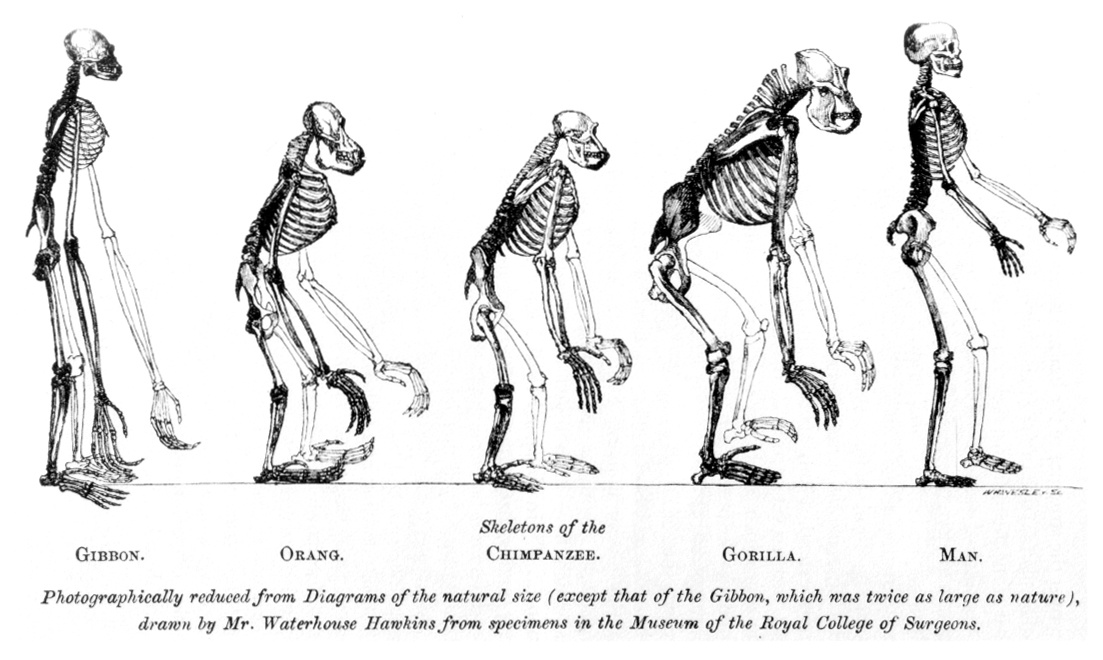
\includegraphics[width = \textwidth]{illustration_images/Genetic_drift/Huxley_mans_place/Huxley_Mans_Place_in_Nature.jpg}
\end{center}
\caption{Illustration by Benjamin Waterhouse Hawkins from Huxley's
  ``Evidence as to Man's Place in Nature'' (1863).
\newline \noindent \tiny{Image from the
  \href{https://en.wikipedia.org/wiki/Pithecometra_principle\#/media/File:Huxley_-_Mans_Place_in_Nature.jpg}{wikimedia},
   public domain.} 
} \label{fig:Huxley_man}
\end{figure}


\section{The Neutral Substitution process.} 
So how then do neutral substitutions occur? It is very unlikely that a rare
neutral allele accidentally drifts up to fixation; more likely, such an allele
will be eventually lost from the population. However, populations experience a
large and constant influx of rare alleles due to mutation, so even if it is
very unlikely that an individual allele fixes within the population, some
neutral alleles will fix by chance. So we'll need to understand the
probability that a neutral mutation fixes, and then how we can think
about the rate of substitutions accumulate over time.\\


%We'll first consider the probability that a neutral allele fixes
%within the population, starting from it just enters a diploid
%population as a newly mutated allele at frequency $1/(2N)$.

%so for an allele to be fixed in the population it
%must have been that allele

\subsection{probability of the eventual fixation of a neutral allele}
% TODO: tried to clean up this section, needs more work
\begin{figure}
\begin{center}
  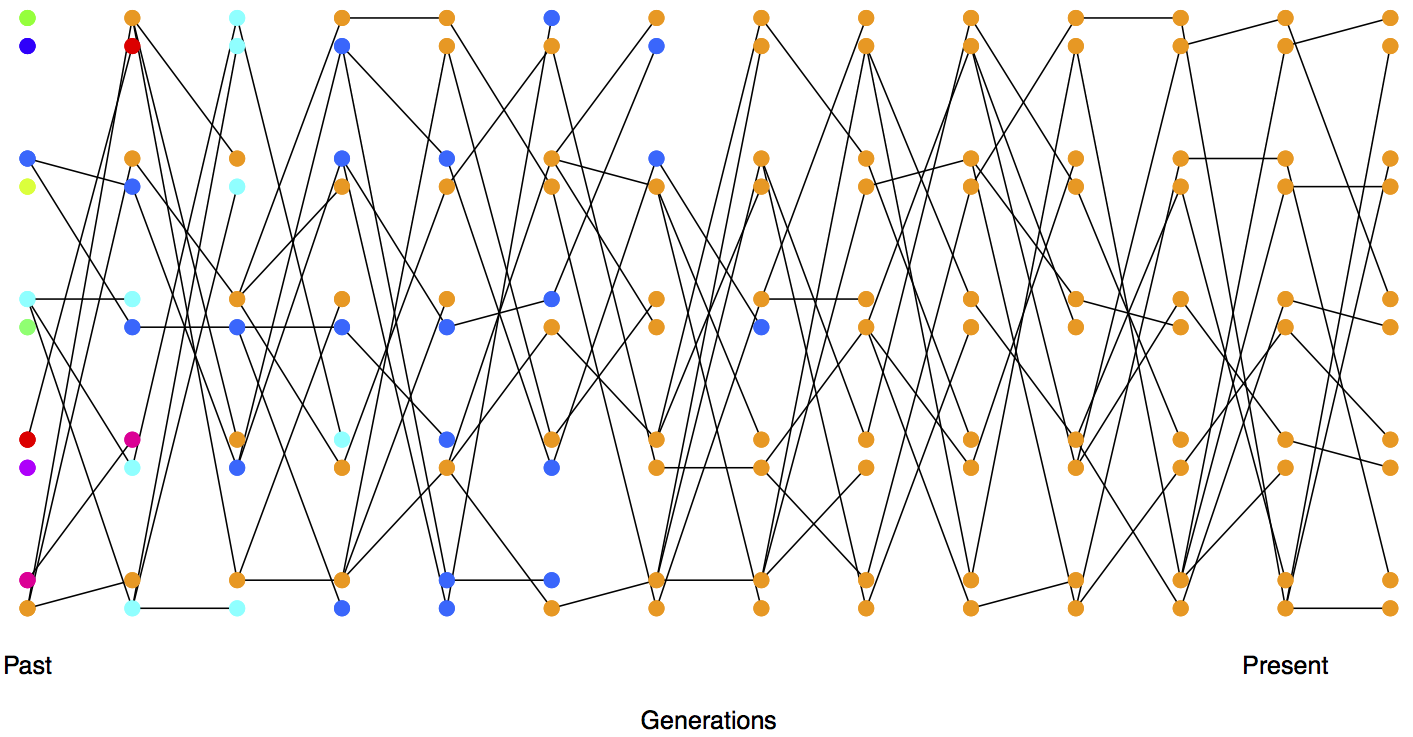
\includegraphics[width = \textwidth]{figures/Substitution_sim.png}
\end{center}
\caption{Each allele initially present in a small diploid population is
  given a different colour so we can track their descendants over
  time. By the 9th generation, all of the alleles present in the
  population can trace their ancestry back to the orange allele. \gitcode{https://github.com/cooplab/popgen-notes/blob/master/Rcode/Loss_of_heterozyg_varying_pop.R}} \label{fig:subs_simulation}
\end{figure}

An allele which reaches fixation within a population is an ancestor to the
entire population. In a particular generation there can only be a single allele
that all other alleles at the locus in a later generation can claim as an
ancestor (See Figure \ref{fig:subs_simulation}). At a neutral locus, the actual allele does not affect the number of
descendants that the allele has (this follows from the definition of
neutrality: neutral alleles don't leave more or less descendants on average than other neutral alleles).
An equivalent way to state this is that the allele labels don't affect
anything; thus the alleles are \emph{exchangeable}. As a consequence of being exchangeable,
any allele is equally likely to be the ancestor of the entire population.  In a
diploid population of size $N$, there are $2N$ alleles, all of which are
equally likely to be the ancestor of the entire population at some later time
point. So if our allele is present in a single copy, the chance that it is the
ancestor to the entire population in some future generation is
$\nicefrac{1}{(2N)}$, i.e. the chance our neutral allele is eventually fixed is
$\nicefrac{1}{(2N)}$.  In Figure \ref{fig:subs_simulation}, our orange allele
in the first generation is one of 10 differently coloured alleles, and so has a
$1/10$ chance of being the ancestor of the entire population at some later time
point (and in this simulation it does become the common ancestor, by the 9th generation).\\

More generally, if our neutral allele is present in $i$ copies in the
population, of $2N$ alleles, the probability that this allele becomes fixed is
$\nicefrac{i}{(2N)}$, i.e. the probability that a neutral allele is eventually
fixed is simply given by its frequency ($p$) in the population.  (We can also
derive this result by letting $Ns \rightarrow 0$ in eqn.
\eqref{eqn:prob_fixed}, a result we'll encounter later.)


% TODO
%A newly arisen mutation only becomes a fixed difference if it is lucky
%enough to be the ancestor of the entire population. As we saw above, this occurs
%with probability $\nicefrac{1}{(2N)}$.

How long does it take on average for
such an allele to fix within our population? In developing
equation \eqref{TMRCA_neutral} we've seen that it takes on average $4N$
generations for a large sample of alleles to all trace their ancestry back to a
single most recent common ancestral allele. Any single-base pair change which arose as a single mutation at a locus, and fixed in the population, must have been present in the sequence transmitted by the most recent common ancestor of the population at that locus. Thus it must take roughly $4N$ generations
for a neutral allele present in a single copy within the population to fix.
 This argument can be made more
precise, but in general we would still find that it takes $\approx 4N$
generations for a neutral allele to go from its introduction to fixation with
the population.   \\

\subsection{Rate of substitution of neutral alleles}

A substitution between populations that do not exchange gene flow is simply a
fixation event within one population. The rate of substitution is therefore the
rate at which new alleles fix in the population, so that the long-term
substitution rate is the rate at which mutations arise that will eventually
become fixed within our population.\\

Let's assume, based on our discussion of the neutral theory of molecular evolution, that there are only two classes of mutational changes that can occur with a
region, highly deleterious mutations and neutral mutations. A fraction $C$ of
all mutational changes are highly deleterious, and cannot possibly contribute
to substitution nor polymorphism.  The other $1-C$ fraction
of mutations are neutral. If our total mutation rate is $\mu$ per transmitted allele
per generation, then a total of $2N \mu (1-C)$ neutral mutations enter our
population each generation.\\

Each of these neutral mutations has a $\nicefrac{1}{(2N)}$ probability chance of
eventually becoming fixed in the population. Therefore, the rate at
which neutral mutations arise that eventually become fixed within our
population is
\begin{equation}
2N\mu(1-C)\frac{1}{2N} = \mu(1-C)
\end{equation}
Thus the rate of substitution, under a model where newly arising alleles are either
highly deleterious or neutral, is simply given by the mutation rate
of neutral alleles, i.e. $\mu(1-C)$.\\

Consider a pair of species that have diverged for $T$ generations, i.e. orthologous sequences shared between the species last shared a common ancestor $T$ generations ago. If these species have maintained a constant $\mu$ over that time, they will have accumulated an average of
\begin{equation}
2\mu(1-C)T \label{eqn:moleclock}
\end{equation}
neutral substitutions. This assumes that $T$ is a lot longer than the time it
takes to fix a neutral allele, such that the total number of
alleles introduced into the population that will eventually fix is the
total number of substitutions.\\

This is a really pretty result as the population size has completely canceled
out of the neutral substitution rate. However, there is another way to see this
in a more straight forward way. If I look at a sequence in me compared to, say, a
particular chimp, I'm looking at the mutations that have occurred in both of
our germlines since they parted ways $T$ generations ago. Since neutral alleles
do not alter the probability of their transmission to the next generation, we
are simply looking at the mutations that have occurred in $2T$ generations
worth of transmissions. Thus the average number of neutral mutational
differences separating our pair of species is simply $2\mu (1-C) T$.\\
%JRI: this is a nice explanation that is not commonly given. Cool.

\subsection{Implications for the Molecular Clock.}
\marginnote{\begin{quote}"Functionally less important molecules or parts of a molecule
evolve faster than more important ones." \end{quote} -- \citet{kimura1974some}}
A number of observations follow under this model, from equation
\eqref{eqn:moleclock}. The first is that a primary determinant of
patterns of molecular evolution in a genomic region is the level of
constraint ($C$). This pattern generally seems to hold empirically:
non-coding regions often evolve more rapidly than coding regions,
synonymous substitutions accumulate faster than nonsynonymous, and
nonsynonymous substitutions accumulate faster in less vital proteins
than ones that are absolutely necessary for early development. For
example, fibrinopeptides evolve in a less constrained manner than the
cytochrome c gene, see Figure \ref{fig:Dickerson_mole_clock}. Note
that this constraint prediction is not a unique prediction of the neutral model, e.g. less constrained regions may also be better able to evolve adaptively. However, it is a fantastically useful general insight, e.g. it allows us to spot putatively functional non-coding regions by looking for genomic regions that have very low levels of divergence among distantly related species.
%JRI: removed mention of pleiotropy as we don't know what it is yet and as far as I can tell there's no mention in rest of book of how pleiotropy relates to constraint
\begin{figure}
\begin{center}
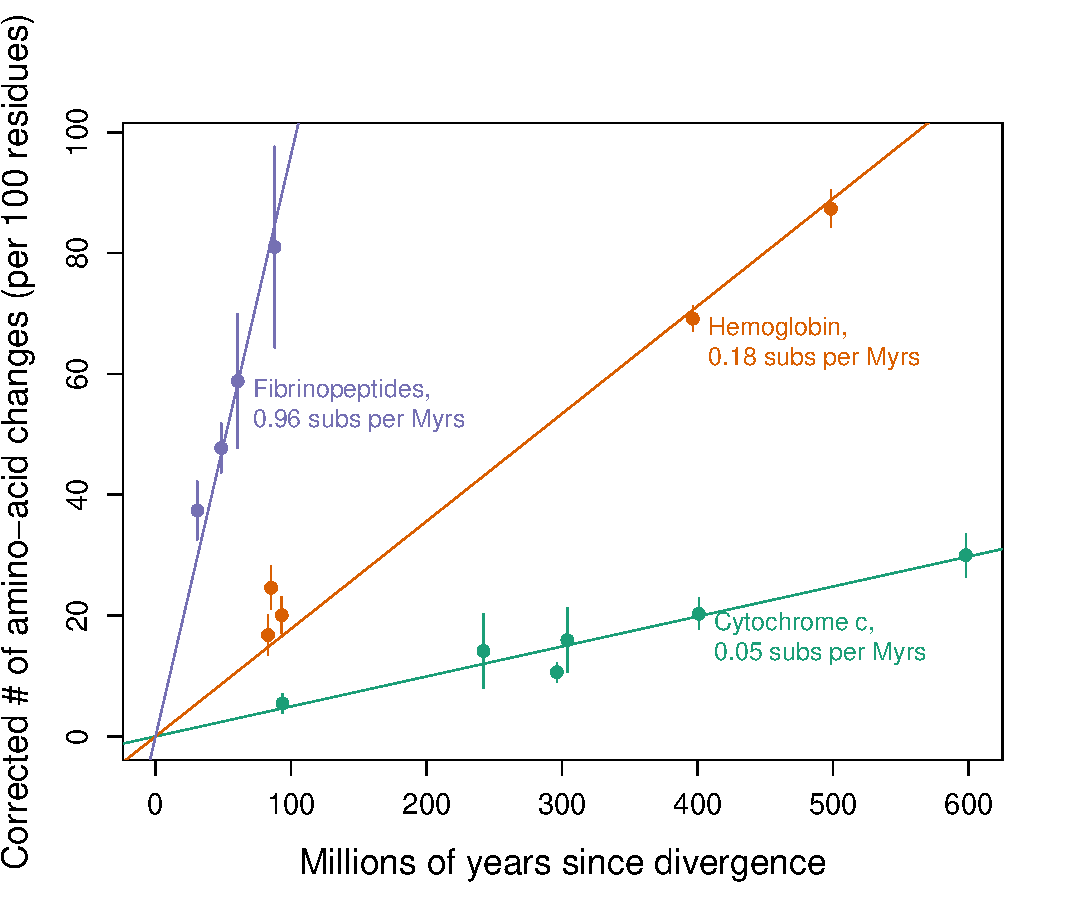
\includegraphics[width=0.8 \textwidth]{Journal_figs/genetic_drift/Molecular_clock_Dickerson/Dickerson_1979_mole_clock_fig.pdf}
\end{center}
\caption[][-2cm]{The numbers of substitutions in three proteins, corrected for multiple hits, between various pairs of groups plotted against the time these groups shared a common ancestor in the fossil record. Data from  \citet{dickerson1971structure}.  The lines give the linear regression through the origin for each protein. The slope of the regression is given next to the protein name. \gitcode{https://github.com/cooplab/popgen-notes/blob/master/Journal_figs/genetic_drift/Molecular_clock_Dickerson/Dickerson_1979_mole_clock_data.R} See \citep{robinson2016revisiting} who revisited this classic study and confirmed the conclusions.} \label{fig:Dickerson_mole_clock}
\end{figure}

\begin{marginfigure}[-2cm]
\begin{center}
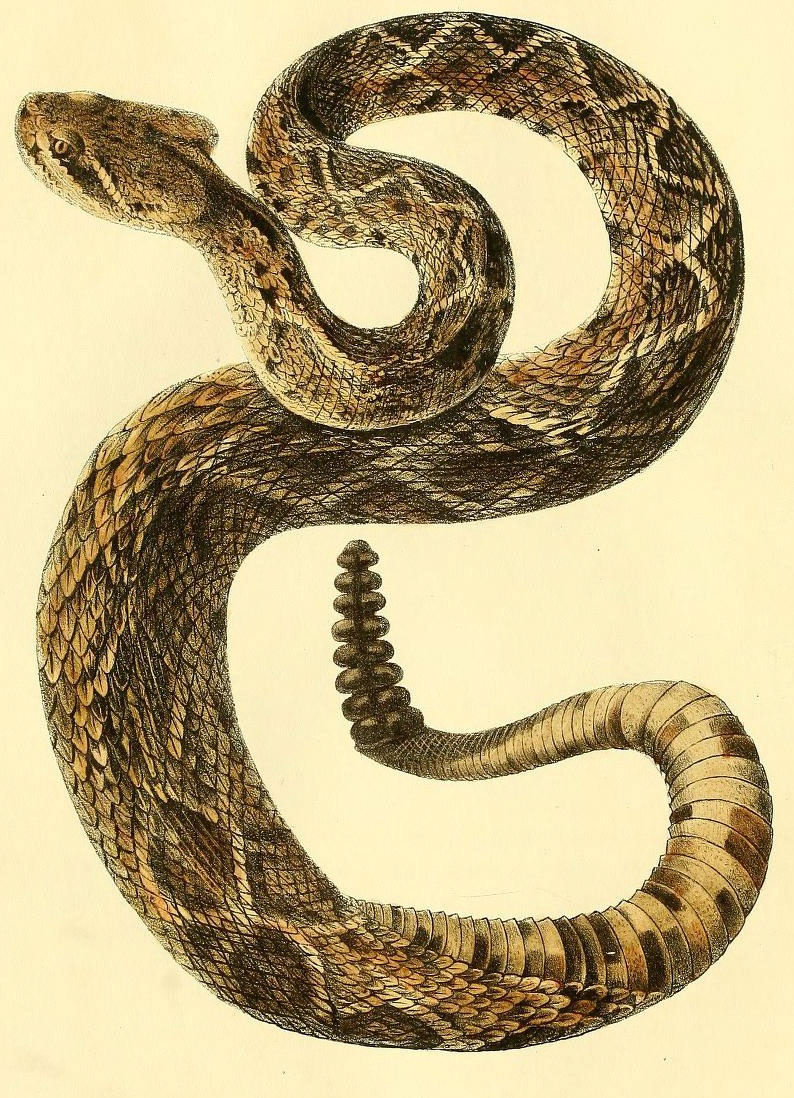
\includegraphics[width= 0.7 \textwidth]{illustration_images/Genetic_drift/rattlesnake/rattlesnake.jpg}
\end{center}
\caption{Eastern diamondback rattlesnake ({\it Crotalus adamanteus}). \BHLCC{North American herpetology. Holbrook, J. E. }{https://www.biodiversitylibrary.org/page/35765722\#page/120/mode/1up}{Smithsonian Libraries}{2.0} } \label{fig:rattlesnake}
\end{marginfigure}



The second important insight, and critical for the development of the neutral theory, is that equation \eqref{eqn:moleclock} is seemingly consistent with \citet{zuckerkandl1965evolutionary}'s hypothesis of a surprisingly constant, protein molecular clock. The protein molecular clock is the observation that for some proteins there's a linear relationship between the number of non-synonymous (NS) substitutions and the time species last shared a common ancestor in the fossil record. \citet{dickerson1971structure} provided an for early example of this observation (Figure \ref{fig:Dickerson_mole_clock}), by comparing various organisms whose molecular sequences were available to him. For example, he found that humans and rattlesnakes, who last share a common ancestor in the fossil record around 300 million years, are separated by roughly $15$ NS substitutions per $100$ sites in the cytochrome c protein.
While, humans and dogfish, which diverged around 400 million years, are separated by $19$ NS substitutions per $100$ sites in this gene. \\ \graham{add dog fish pic? https://www.flickr.com/photos/biodivlibrary/sets/72157645618396122/ Added molecular clock question}

\begin{marginfigure}
\begin{center}
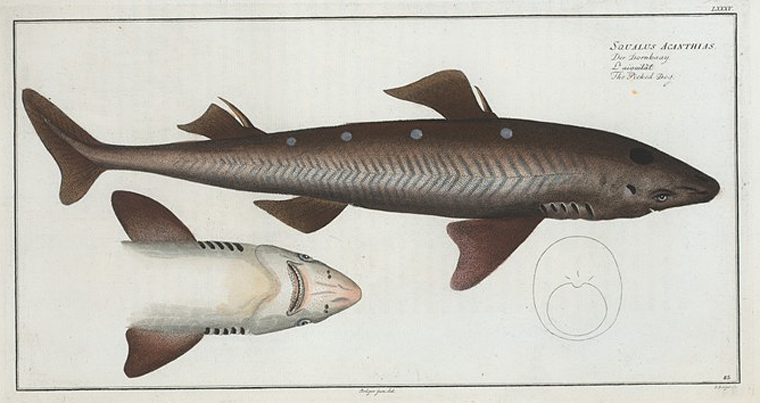
\includegraphics[width= \textwidth]{illustration_images/Genetic_drift/dogfish/dogfish.jpg}
\end{center}
\caption{Spiny dogfish ({\it Squalus acanthias}). \newline \noindent \tiny{ \href{http://digitalcollections.nypl.org/items/510d47da-6930-a3d9-e040-e00a18064a99}{Rare Book Division, The New York Public Library. ``Squalus Acanthias, The Picked- Dog'' The New York Public Library Digital Collections. 1785. Public domain.}}}
\label{fig:dogfish}
\end{marginfigure}

In equation \eqref{eqn:moleclock}, if we double the amount of time separating a pair of species $T$, we double the number of substitutions predicted. Note that for this to be true $T$ must be measured in generations. To explain a protein molecular clock between species that clearly differed dramatically in generation time it was hypothesized that the mutation rate actually scaled with generation time, i.e. short-lived organisms introduced fewer mutations per generation, e.g. as they had fewer rounds of mitosis. This generation-time assumption meant that the mutation rate per year could be constant, such that $\mu T$ would be a constant for pairs of species that had diverged for similar geological times, which are measured in years, even if the organisms differed in generation time. This assumption would allow neutral theory to be consistent with a protein molecular clock measured in years. We now know that this critical generation time assumption is false: organisms with shorter generation times have somewhat higher mutation rates per year so a strict neutral model is inconsistent with the protein molecular clock. We'll return to these ideas when we discuss the fate of very weakly selected mutations in Chapter \ref{Selection_Stochasticity} and \citet{ohta1973slightly}'s Nearly Neutral theory. If you are still reading this send Graham a picture of Tomoko Ohta receiving the Crafoord Prize, an analog of the Nobel prize for biology, for her contributions to molecular evolution.
%JRI: one to many cute send the prof a photo for a single chapter
% graham{I currently dont do generation time effect in that chapter, need to update}
%\graham{add side note on adjustment for multiple hits'}
%\graham{add note about fibrinogen having non-essential spacer pepitides}


\paragraph{The contribution of ancestral polymorphism to divergence.} If we are considering $T$ to represent the divergence between long-separated species, then we can think of $T$ as the time that the
species split. However, for more recently diverged populations and
species, we need to include the fact that the sorting of ancestral
polymorphism contributes to divergence among species. In Figure
\ref{fig:split_anc_pop}, we see our two populations split $T_s$ generations ago.  However, the
coalescence of our A and B lineage is necessarily deeper in time than
$T_s$. The top mutation was polymorphic in the ancestral population
but now contributes to the divergence between A and B. Assuming that
our ancestral population had effective size $N_A$ individuals, and
that our populations split cleanly with no subsequent gene flow, then
\begin{equation}
T = T_s + 2N_A.
\end{equation}
If our species split time is very large compared to $2N$ then we can think of $T$ as the split time.
%JRI: should clarify that above equation only holds only for two lineages. maybe add as a margin note
\begin{marginfigure}
\begin{center}
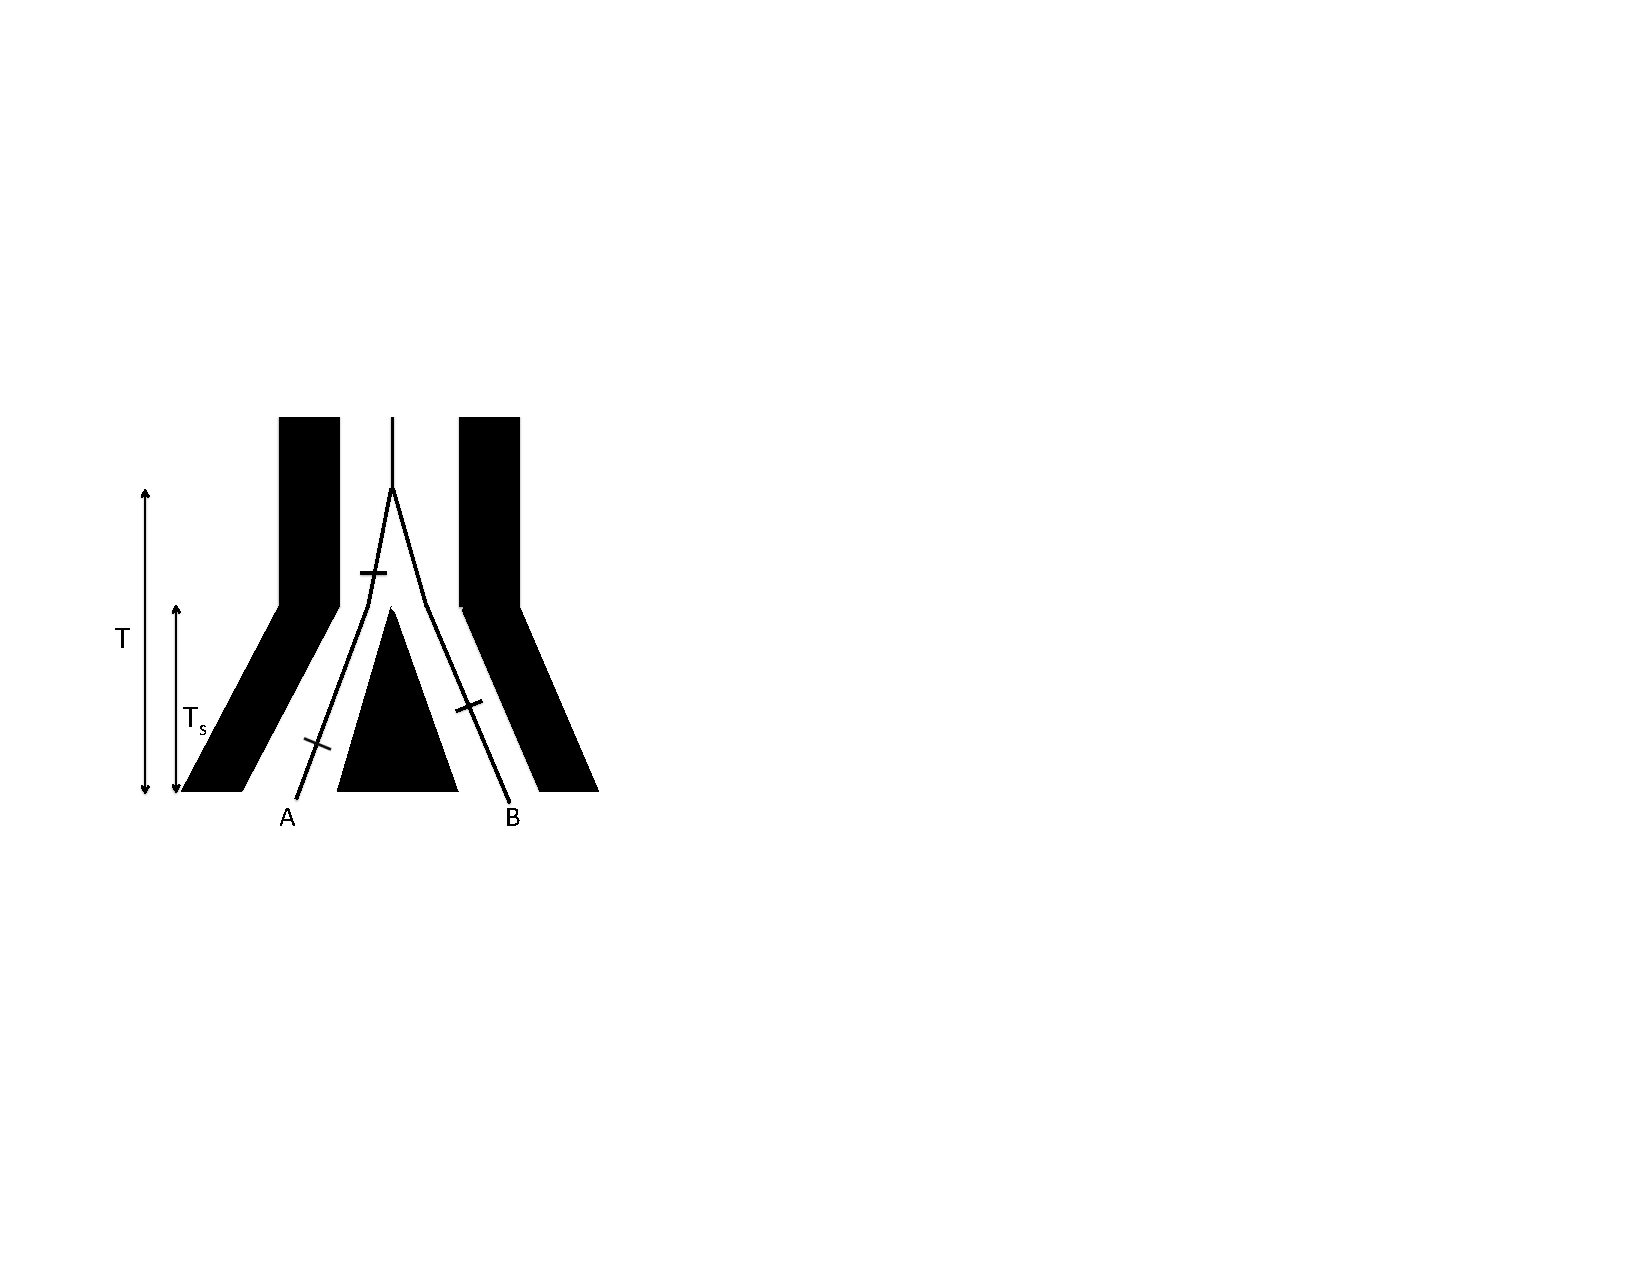
\includegraphics[width=0.8 \textwidth]{figures/Genetic_drift/ILS/split_anc_pop.pdf}
\end{center}
\caption{The genealogy of two alleles one sampled from population A and B. Mutations on the lineages are shown as dashes. The pair of alleles coalesce in the ancestral population of A and B. The two populations split $T_S$ generations ago, with no subsequent gene flow, but the two lineages must coalesce deeper in time. } \label{fig:split_anc_pop}
\end{marginfigure}

\graham{update numbers in Q}
%Our expected number of substitutions is scaling linearly with our species $T$ split time measured in generations.

%\erin{I think this last concept is hard and may be a bit confusing for students without some additional pictures or text} %\graham{lineup split time in this section w. FST section.}



\begin{question}{}
For this, and the next question, assume that humans and chimps split
%\graham{Update numbers?}
around 5.5$\times 10^6$ years ago, have a generation time ~20 years, that the speciation occurred instantaneously in allopatry with no subsequent gene flow, and the ancestral effective population size of the human and chimp common ancestor population was 10,000 individuals.\\
Nachman and Crowell sequenced 12 pseudogenes in humans and chimps and found substitutions at 1.3\% of sites. \\
{\bf A) } What is the mutation rate per site per generation at these genes?\\
{\bf B)} All of the pseudogenes they sequenced are on the autosomes. What
would your prediction be for pseudogenes on the X and Y chromosomes,
given that few mutations occur in the female
germline than in the male germline per generation.
\end{question}

\section{Tests of molecular evolution.}
One of the great appeals of neutral models is they offer a simple null
for us to test real data against. 
\subsection{Comparing the rates of non-synonymous to synonymous
substitutions $\dNdS$}
One common tool in molecular evolution is to compare the estimated
number (or rates) of substitutions in different classes of genomic
sites, for example the ratio of the rates of non-synonymous ($d_N$) to
synonymous substitutions ($d_S$) in a given gene. The simplest way to
think about calculating $d_N$ is to
count up the non-synonymous changes and divide by the total number of
positions in the gene where a non-synonymous point mutation could
occur and then divide by time. We
can do likewise for synonymous changes $d_S$, and then take the ratio $\dNdS$.
\sidenote{This
ignores the fact that some changes are more likely to occur by
mutation than others and also does not account for multiple hits (multiple mutations at the same bp position). Therefore, in
practice the ratio $\dNdS$ is more typically calculated by model-based
likelihood and bayesian methods
that can account for these features.}

For the vast majority of protein-coding genes in the genome we see that $\dNdS < 1$. This observation is consistent with the view
that non-synonymous sites are much more constrained than synonymous sites, i.e. that most non-synonymous mutations are deleterious and quickly removed from the population. If we are willing to make the assumption that all synonymous changes are
neutral, $d_S= \mu$, then we can estimate the degree of constraint on non-synonymous sites. (Note that synonymous changes can sometimes be subject to
both positive and negative selection, but this neutral assumption is a useful starting place.)

Assume that a fraction $C$ of non-synonymous changes are too
deleterious to contribute to divergence, and that there are no
beneficial mutations. Then, %after $T$ generations of divergence have
%elapsed between two populations, we'd
we expected rate of neutral non-synonymous substitutions is
\begin{equation}
d_N = (1-C) \mu
\end{equation}
Dividing by $d_S$, we find
\begin{equation}
\dNdS = (1-C)
\end{equation}
Therefore, if we assume that non-synonymous mutations can only be
strongly deleterious or neutral, we estimate the fraction of mutational changes that
are constrained by negative selection as $C= 1- \dNdS$. C has the
interpretations of being the fraction of non-synonymous mutations that are quickly weeded out of the population by selection, and so do not contribute to divergence among species.

We can test whether our gene is evolving in a constrained way at the protein level by estimating $\dNdS$ and testing whether this is significantly less that  $1$. A $\dNdS$ test can provide evolutionary evidence that a stretch of DNA proposed to be protein-coding is subject to selective constraint, and so likely does encode for a functional protein. We can also perform a $\dNdS$ test on specific branches of a phylogeny for a gene, to test on which branches the gene is subject to constraint, or to test for changes in the level of constraint across the phylogeny.

\graham{add pic of distribution of dN/dS}

\paragraph{Loss of constraint at pseudogenes.}


\marginnote{
``Rudimentary organs may be compared with the letters in a word, still
retained in the spelling, but become useless in the pronunciation, but
which serve as a clue .. for its derivation.''  -- \citet{darwin1859} pg. 455
}  %http://darwin-online.org.uk/Variorum/1859/1859-456-dns.html

While most protein genes evolve under constraint, we can find examples of
genes that are evolving in a much less constrained manner. The simplest
example of this is where the gene has lost function. Genes can lose function because of inactivating mutations that stop them being transcribed or translated into functional proteins. Such genes are called `pseudogenes'.
%JRI: odd to define pseudogene here when you've used the term lots previously
When a gene completely loses function there is no longer
selection against non-synonynous changes and so such mutations are just as free
to accumulate as synonymous changes, and so $\dNdS=1$.
Pseudogenes are a wonderful example of the extension of Darwin's ideas about vestigial traits (`Rudimentary organs') to the DNA level;
we can still recognize a once useful word (gene) whose spelling is slowly degrading. Our genomes are filled with old pseudogenes whose
original meanings (functional protein coding sequences) are slowly being eroded through the accumulation of neutral substitutions.
One nice example of a gene that has repeatedly lost function,
i.e. become repeatedly psuedogenized, is
the {\it enamlin} gene from the study of \citet{Meredith:09}.

\begin{figure}
\begin{center}
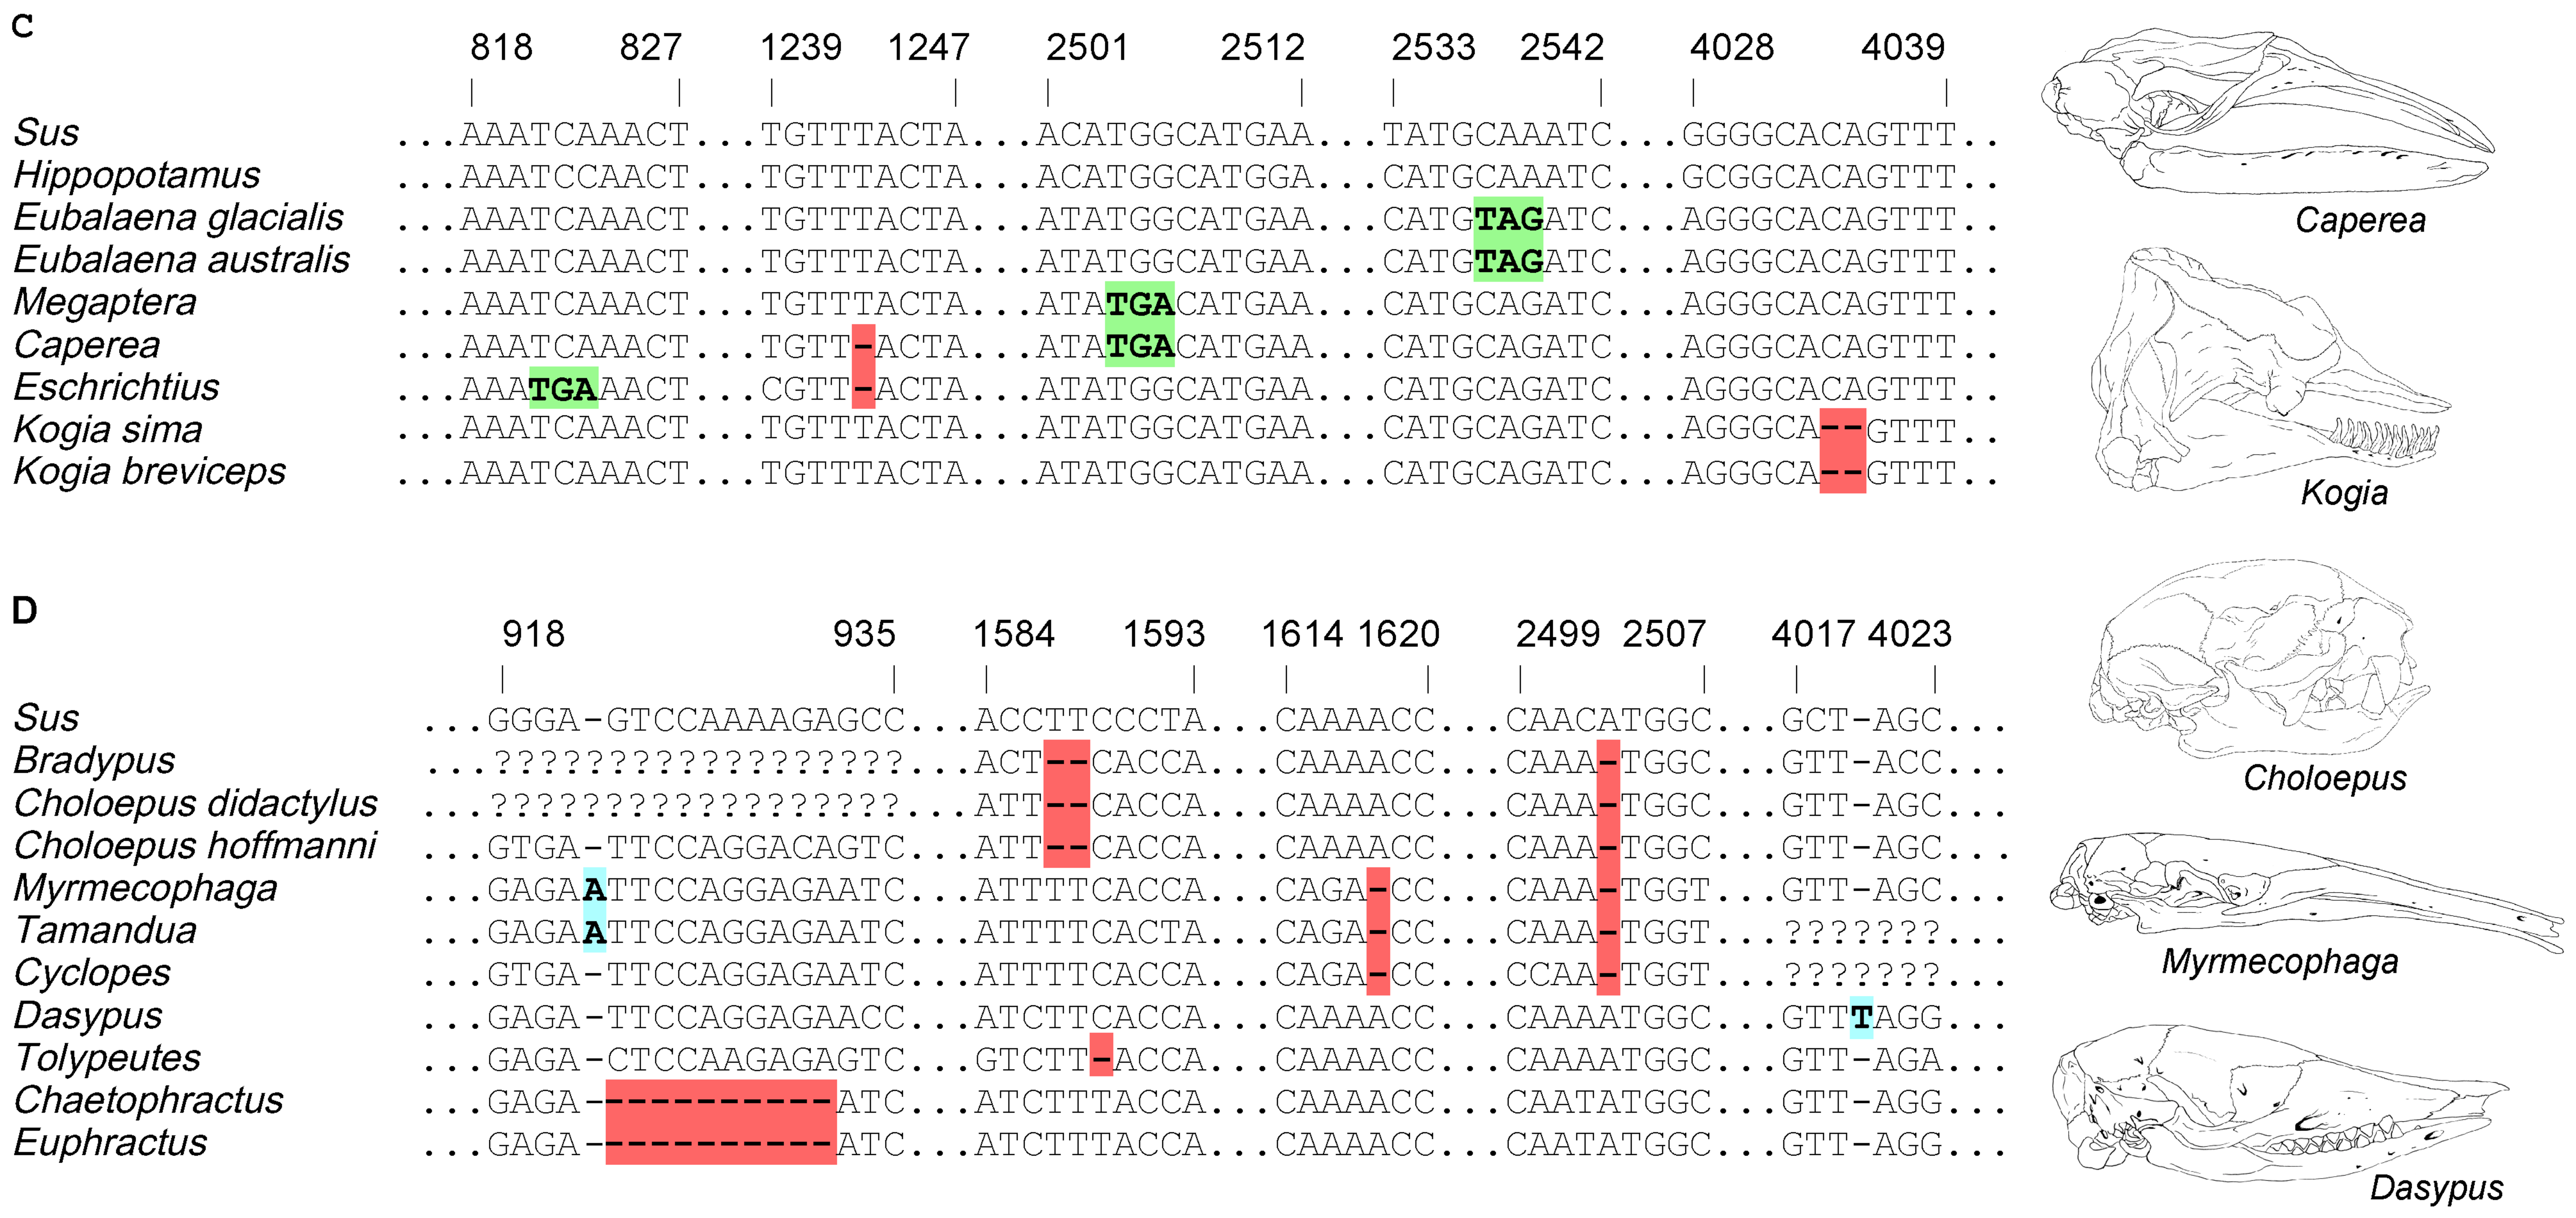
\includegraphics[width=\textwidth]{Journal_figs/genetic_drift/Enamelin/Enamlin.pdf}
\end{center}
\caption{Examples of frameshift mutations (insertions blue, deletions
  red) and premature stop codons in {\it enamlin} in Cetacea and
  Xenarthra. Figure from \citet{Meredith:09}, \PLOSccBY. } \label{fig:Enamlin_coding}
\end{figure}

\begin{marginfigure}
\begin{center}
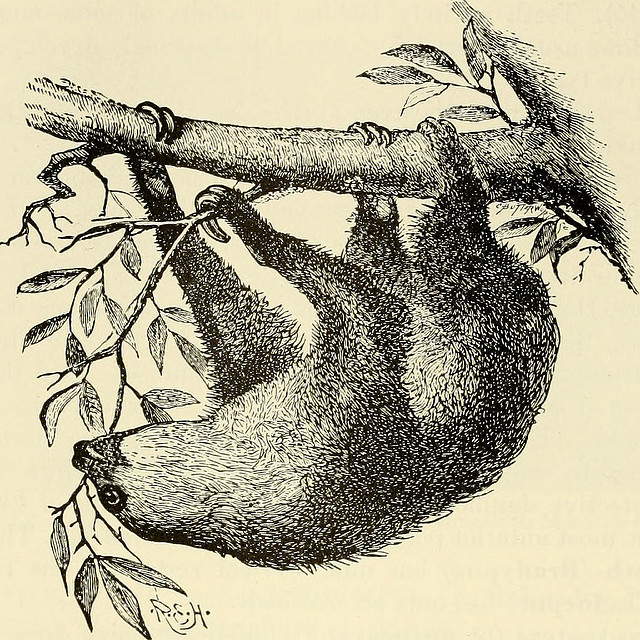
\includegraphics[width=\textwidth]{illustration_images/Genetic_drift/sloth/20423856040_6e4360df9c_z.jpg}   %https://www.biodiversitylibrary.org/page/39742681#page/1005/mode/1up
\end{center}
\caption{Two-toed sloth ({\it Choloepus hoffmanni}). \BHLNC{An introduction
  to the study of mammals, living and extinct. 1891. Flower W. H. and Lydekker R.}{https://archive.org/stream/chordates00rand/\#page/744/mode/1up}{University of Toronto} } \label{fig:sloth}
\end{marginfigure}

The protein {\it enamlin} is a key structural protein involved in the outer cap of enamel on teeth. Various mammals have secondarily evolved diets that do not require hard teeth, and so greatly reduced the selection pressure for hard enamel, or even teeth at all. For example, two-toed sloths ({\it Choloepus}), pygmy sperm whales ({\it Kogia}), and aardvark ({\it Orycteropus}) all lack  enamel on teeth.
%JRI: i don't understand when you choose to capitalize parts of common names of species. Pygmy sperm whale but two-toed sloth. throughout chapters varies a lot
Other mammals have lost their teeth entirely, e.g. giant anteaters
({\it Myrmecophaga}) and baleen whales. Due to this relaxation of
constraint on the phenotype, the {\it enamlin} gene has accumulated pseudogenizing substitutions such as premature stop codons and frameshift mutations (see Figure \ref{fig:Enamlin_coding}
for examples).  \citet{Meredith:09} sequenced {\it enamlin} across a
range of species and found that none of the species with enamel have frameshift
mutations in {\it enamlin}, while 17/20 of species that lack enamel or teeth have
frameshifts in {\it enamlin}, and all of them carry premature stop codons. 
%(Figure \ref{fig:Enamlin_phylo}).

%\begin{figure}
%\begin{center}
%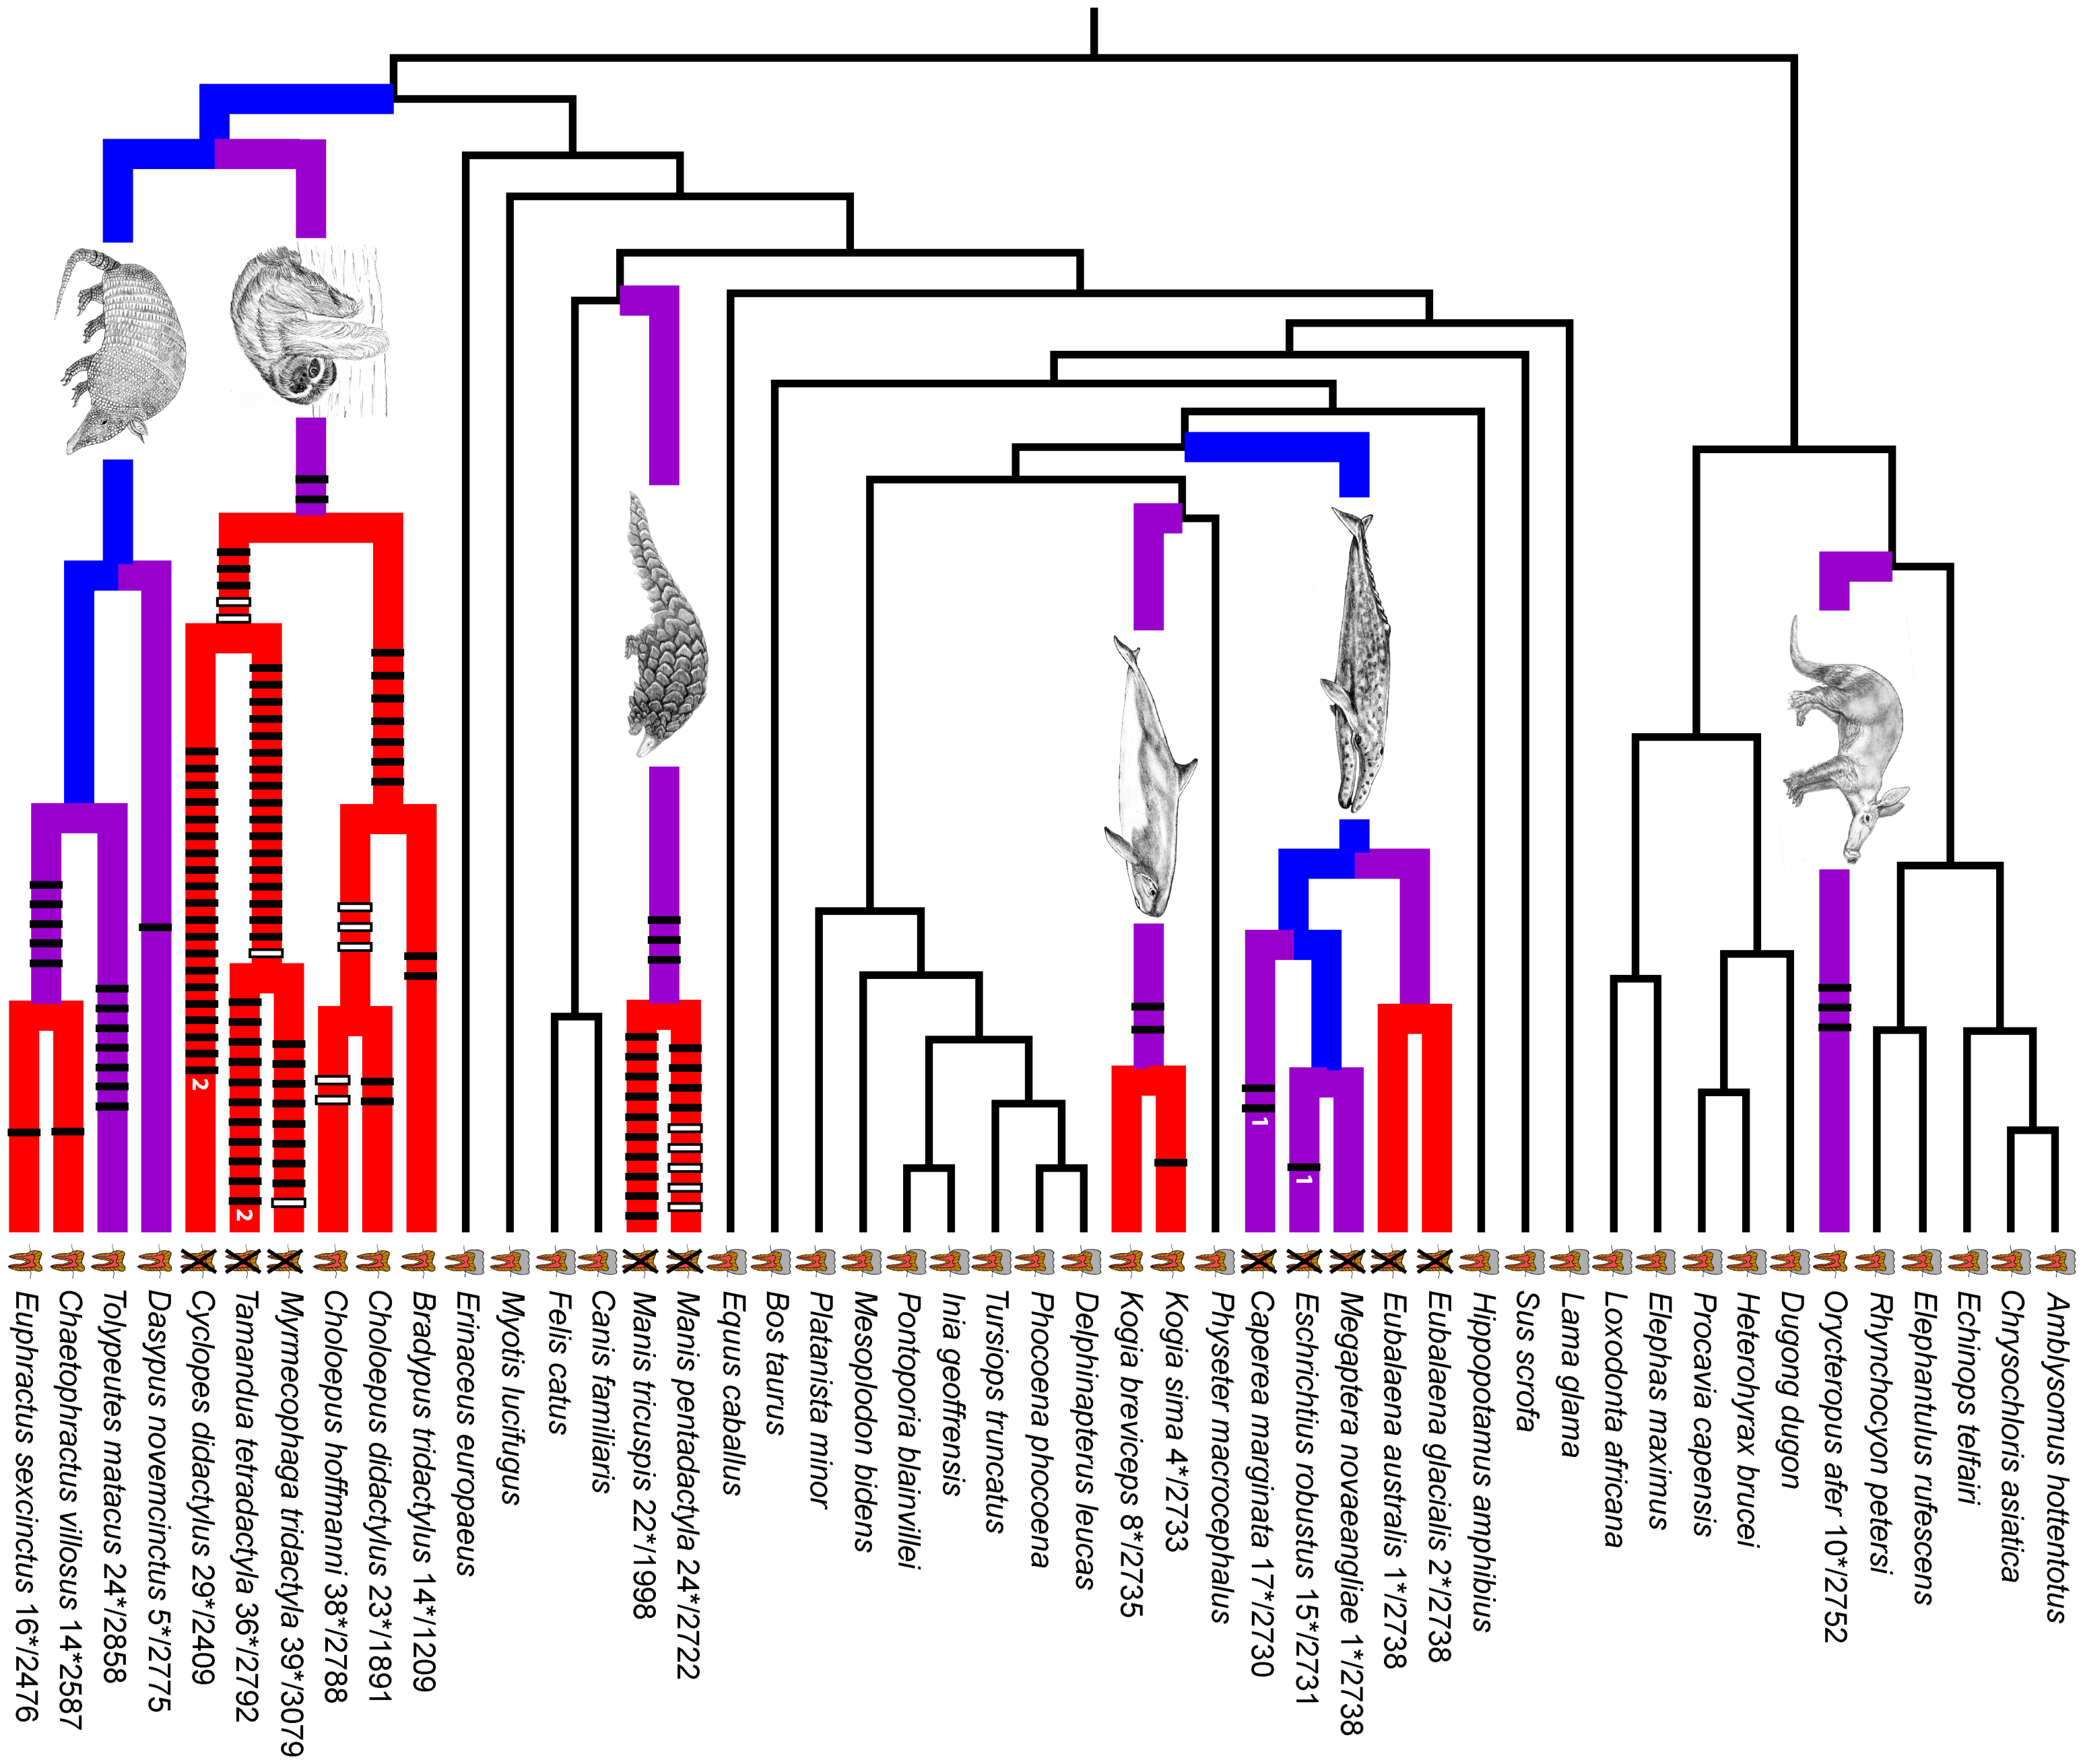
\includegraphics[width= \textwidth]{Journal_figs/genetic_drift/Enamelin/Enamlin_phylo.pdf}
%\end{center}
%\caption{The tooth symbol next to each taxon shows whether they have
 % teeth with enamel, lack enamel, or lack teeth. Branches of the phylogeny are coloured by whether their
 % Enamlin is functional (black), pre-mutation (blue), mixed (purple), or pseudogenic (red). The black and white  bars on branches show frameshift
 % mutations.  The numbers after taxon names indicate minimum number of
 % stop codons in the sequence divided by  the length of the sequence. Figure from \citet{Meredith:09}, \PLOSccBY.} \label{fig:Enamlin_phylo}
%\end{figure}
%JRI: recommend removing or editing this. i had to zoom in a lot to figure out the teeth, the numbers aren't easy to read, etc.  not a helpful figure

 \citet{Meredith:09} found that the branches of the {\it enamlin}
 phylogeny with a functional {\it enamlin} gene %(black) 
had an estimated $\dNdS= 0.51$, consistent with the protein
evolving in a constrained manner. In contrast, the branches with a
pseudogenized Enamlin % (red)
had $\dNdS = 1.02$, consistent with the gene evolving a completely unconstrained
way. The branches where the gene was likely transitioning from a functional
to non-function state, i.e. pre-mutation % (blue)
and mixed, %purple),
had intermediate values of
$\dNdS=0.83-0.98$, consistent with a transition from a constrained to unconstrained mode of protein evolution somewhere along these branches of the phylogeny.

\begin{figure}
\begin{center}
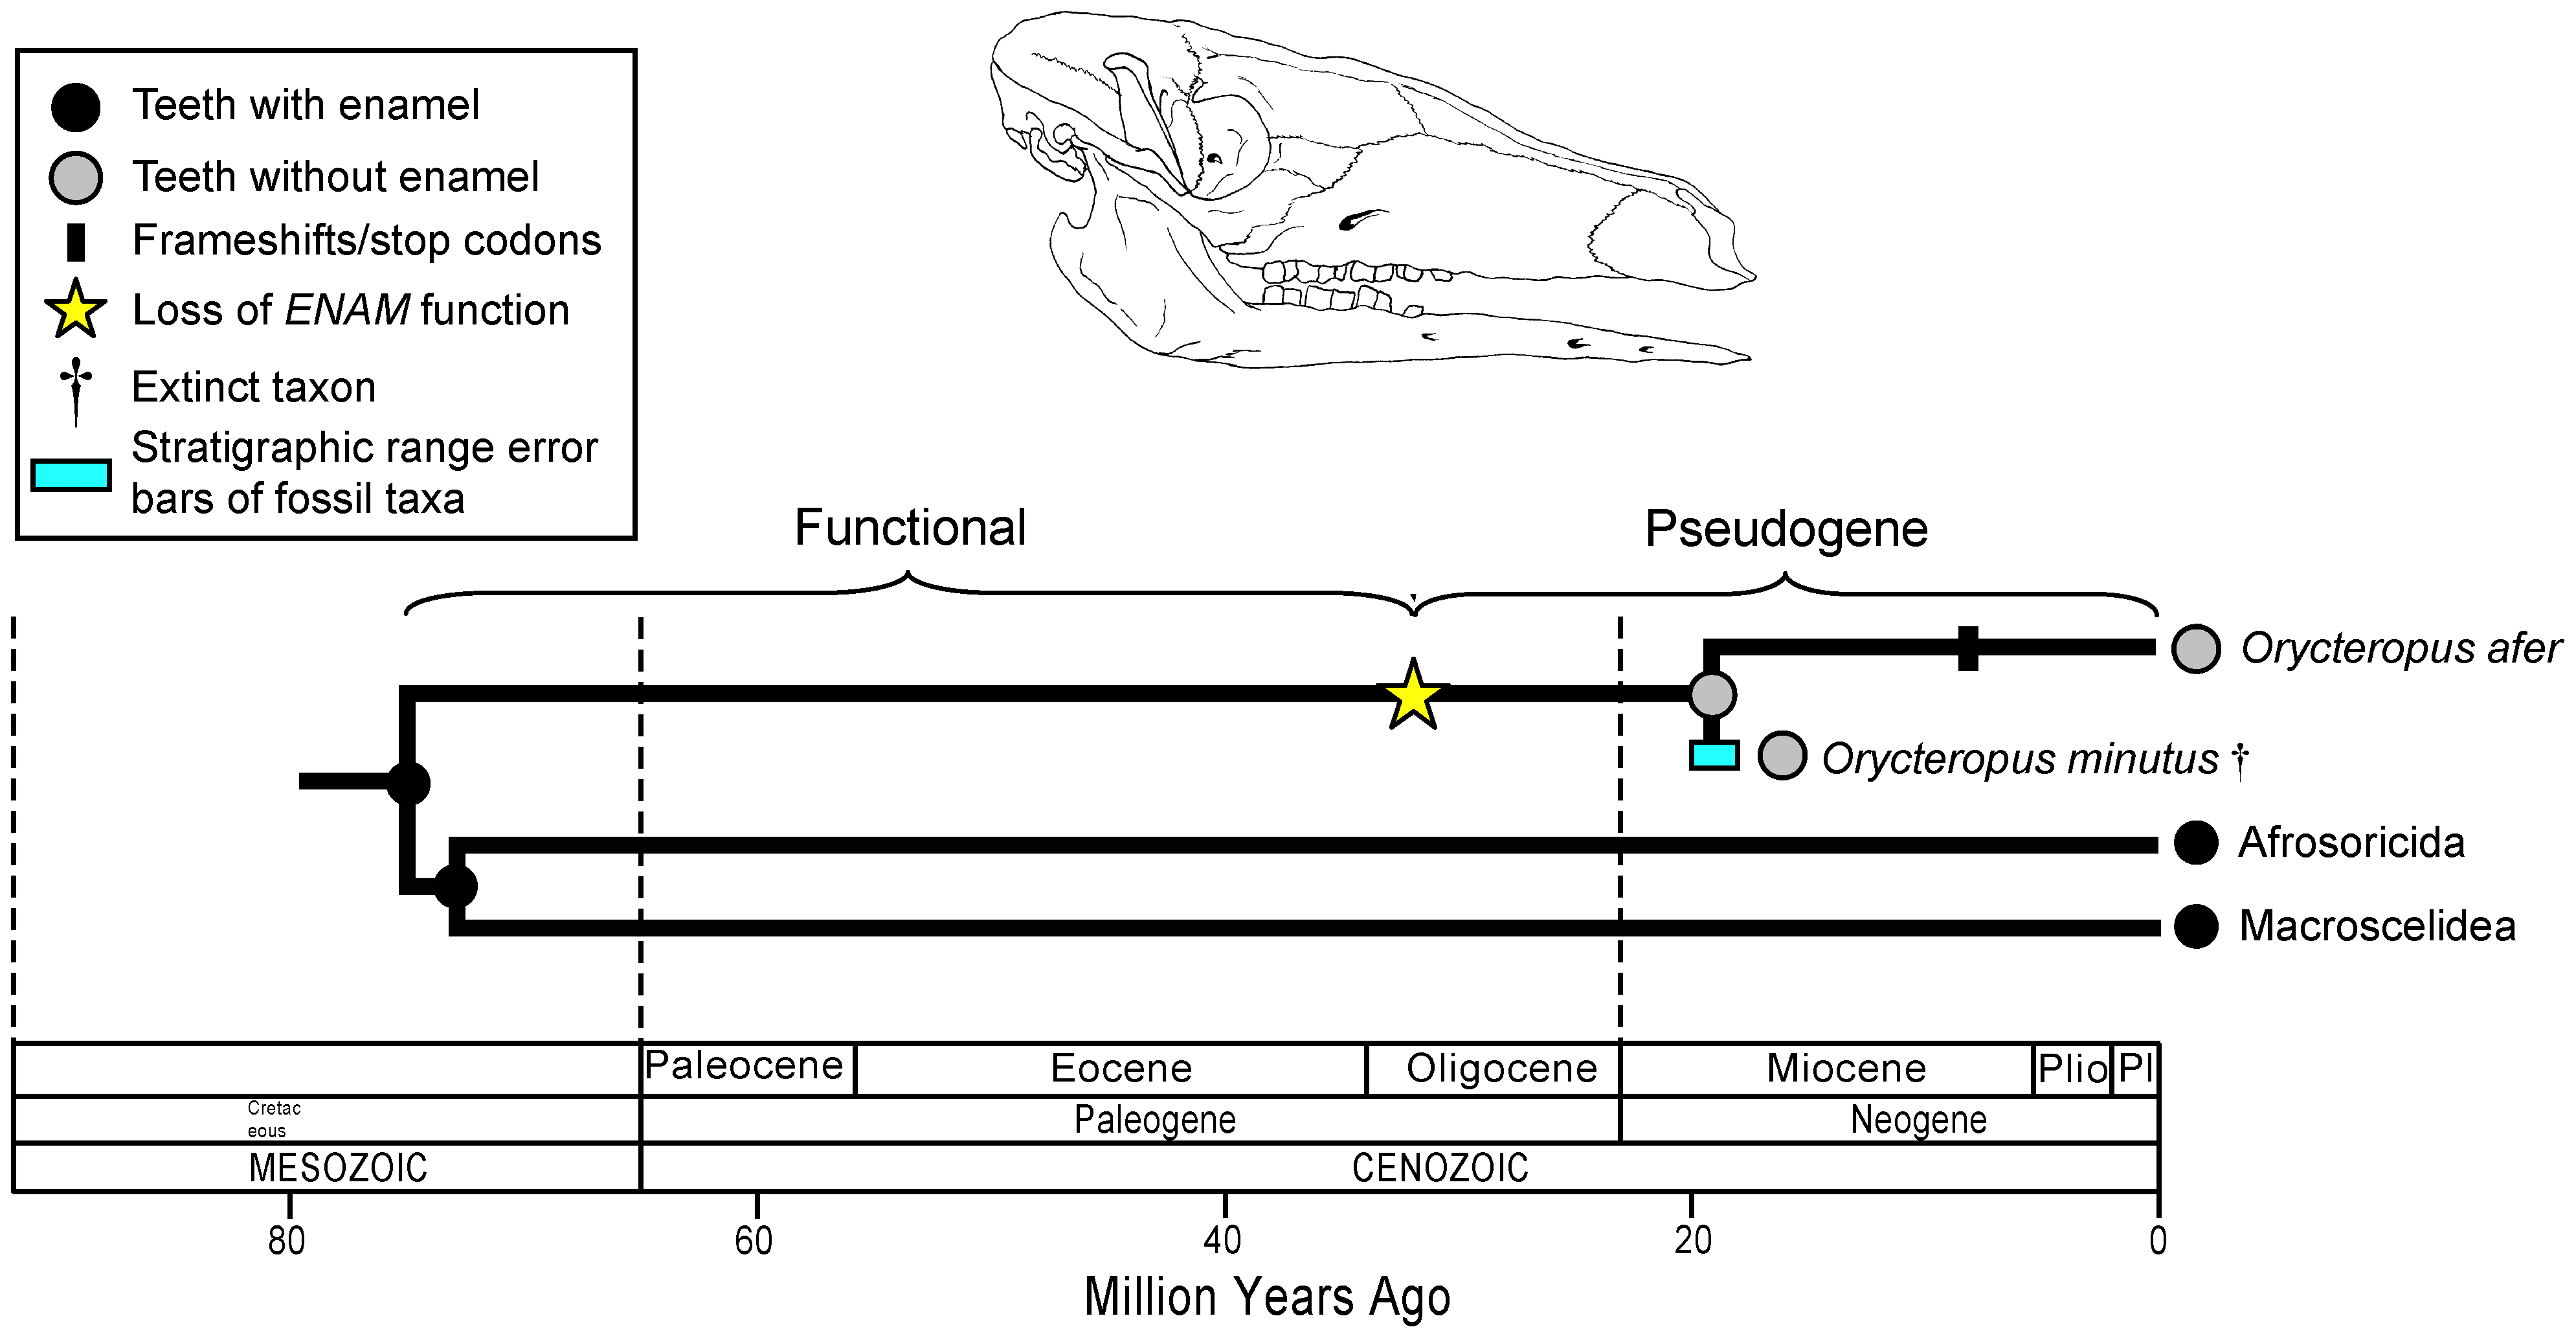
\includegraphics[width=\textwidth]{Journal_figs/genetic_drift/Enamelin/Aardvark_pseudogene.png}
\end{center}
\caption{ A synthetic interpretation of the history of enamel
  degeneration in {\it Tubulidentata} (the order of aardvarks) based on fossils,
  phylogenetics, molecular clocks, frameshift mutations, and $\dNdS
$  ratios. The oldest fossil aardvarks are {\it O. minutus} (19 mya) from the
  early Miocene of Kenya and also lack enamel.  Figure \& caption modified from
  \citet{Meredith:09}, \PLOSccBY. } \label{fig:Aardvark_pseudogene}
\end{figure}


\begin{marginfigure}
\begin{center}
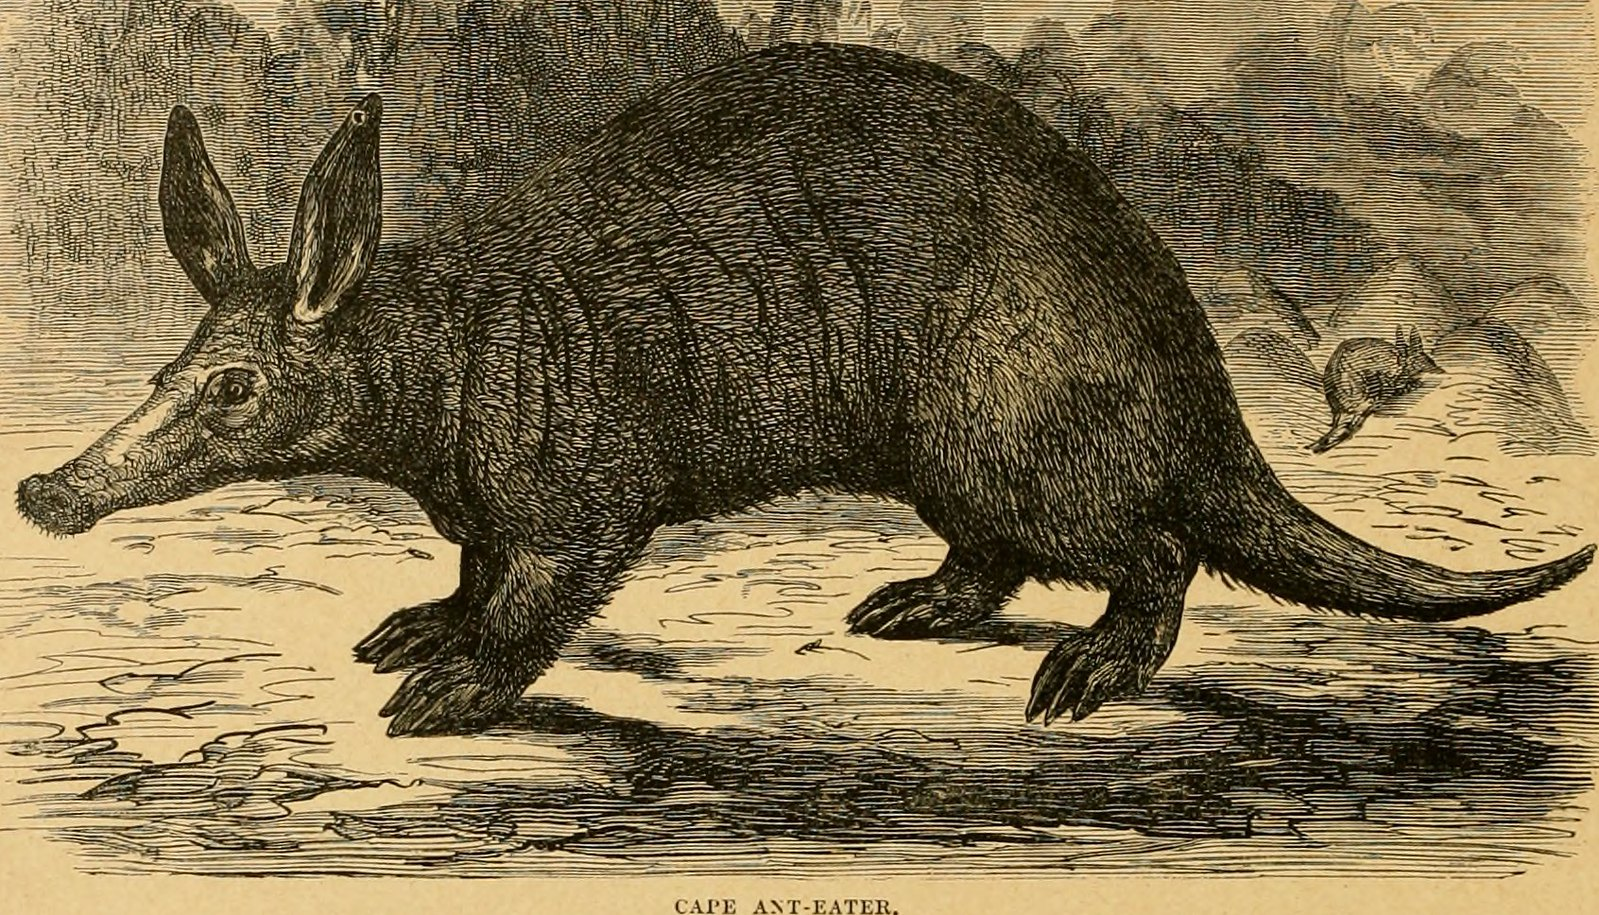
\includegraphics[width=\textwidth]{illustration_images/Genetic_drift/aardvark/20514695666_5a22b53b8c_h.jpg}
\end{center}
\caption{Aardvarks (Cape ant-eater, {\it Orycteropus afer}) \BHLNC{Cassell's natural history ( 1896 ).  Duncan, P. M.}{https://www.flickr.com/photos/internetarchivebookimages/20514695666/in/photolist-xfPbiq-xUcng7-xCyGQA-xdRRQ3-wPMGZr-tFgYfN-wPMPkT-tDahHQ-xuc4KM-xKR4u3-xUkupQ-w88zeU-xMia2r-sp4Aq5-x1wNyZ-xMi46D-tDaCr7-sJE2X4-tFB8Lc-wHWiNj-tp8AUk-tFvh4R-xu3M7w-toUVwN-wYWgVi-w34vHn-x9xAfL-wWhnso-ovvmHE-tG5AgB-xdUzWD-y82dEG-xCA7kx-xV5xWg-wYc33H-wYbFdX-wYbBMP-xUcjpL-xKQjHw-xJmBQU-xKPwEQ-xLEzv4-xu3wHJ-xLEg9V-xnA6Lr-x684wQ-wZNgpq-wYcVbh-wZtb3F-wYbJLh}{NCSU Libraries}} \label{fig:Aardvark}
\end{marginfigure}
\begin{question}{}
The {\it enamlin} gene was pseudogenized somewhere along the branch leading to
Aardvarks ({\it Orycteropus afer}), see Figure
\ref{fig:Aardvark_pseudogene}. \citet{Meredith:09} estimated that this
branch has a $\dNdS=0.75$\\
{\bf A)} Calculate the average constraint against amino-acid changes
on this branch.\\

{\bf B)} Aardvarks last shared a common ancestor
with {\it Afrosoricida} (golden moles, tenrecs) and {\it Macroscelidea} (elephant
shrews) around $\sim 75.1$ million years ago in the Cretaceous. Assume
that for the portion of the branch while
{\it enamlin} was functional $\dNdS = 0.51$  and
after it was pseudogenized there was no constaint (i.e. $\dNdS = 1$). Based on the branch's average $\dNdS=0.75$, can
you estimate the time at which {\it enamlin} was pseudogenized? (I.e. when
is the star in Figure \ref{fig:Aardvark_pseudogene}?)
% https://journals.plos.org/plosgenetics/article?id=10.1371/journal.pgen.1000634#pgen.1000634.s007
%dawn pangloin
%https://commons.wikimedia.org/wiki/File:Eomanis_waldi_4.jpg
%% aadvark https://www.flickr.com/photos/internetarchivebookimages/20514695666/in/photolist-xfPbiq-xUcng7-xCyGQA-xdRRQ3-wPMGZr-tFgYfN-wPMPkT-tDahHQ-xuc4KM-xKR4u3-xUkupQ-w88zeU-xMia2r-sp4Aq5-x1wNyZ-xMi46D-tDaCr7-sJE2X4-tFB8Lc-wHWiNj-tp8AUk-tFvh4R-xu3M7w-toUVwN-wYWgVi-w34vHn-x9xAfL-wWhnso-ovvmHE-tG5AgB-xdUzWD-y82dEG-xCA7kx-xV5xWg-wYc33H-wYbFdX-wYbBMP-xUcjpL-xKQjHw-xJmBQU-xKPwEQ-xLEzv4-xu3wHJ-xLEg9V-xnA6Lr-x684wQ-wZNgpq-wYcVbh-wZtb3F-wYbJLh
%%% w1 t/T + w2(T-t)/T = wT
%% https://journals.plos.org/plosgenetics/article?id=10.1371/journal.pgen.1000634#pgen.1000634.s007
\end{question}
\paragraph{Adaptive evolution and $\dNdS$.}
Clearly genes are not only subject to neutral and deleterious mutations; beneficial mutations must also arise and fix from from time to time.
Let's assume that a fraction $B$ of non-synonymous mutations that arise are
beneficial such that $2 N \mu B$ beneficial mutations arise per generation. Newly arisen beneficial alleles are not destined to fix in the population, as they may be lost to genetic drift when they are rare in the population (we'll
discuss how to calculate the fixation probability for beneficial
alleles in Chapter \ref{Selection_Stochasticity}). A newly arisen beneficial allele reaches fixation in the population with probability $f_B$ from its initial frequency of $\nicefrac{1}{2N}$. This fixation
probability may be much higher than that of neutral mutations, but
still much less than $1$. The expected total rate of non-synonymous
substitutions is
%If $2T$ generations of divergence have
%elapsed between the two populations then a total of
\begin{equation}
dN= (1-C - B) \mu  +   (2 N \mu B) \times  f_B.
\end{equation}
Then
\begin{equation}
\dNdS = (1-C-B) +  2 N B f_B \label{eqn:dNDS_C_B}
\end{equation}
assuming again that all synonymous mutations are neutral. Note that this means that our estimates of $C$ using $1-\dNdS$ will be
a  lower bound on the true constraint if even a small fraction of
mutations are beneficial. Those cases where the gene is evolving more rapidly at the protein level than at synonymous
sites, i.e. $d_N/d_S > 1$, are potentially strong candidates for  positive selection rapidly driving change at the protein level. We can identify genes that have $\dNdS$ significantly greater than one, either on the complete gene phylogeny, or on particular branches. Note that is a very conservative test that few genes in the genome meet, as many genes that are fixing adaptive non-synonymous substitutions will have $\dNdS<1$;  even if adaptive mutations are common, genes may still evolve in a constrained way (i.e. $\dNdS<1$) if
the rapid fixation of beneficial mutations due to positive selection is outweighed by the loss of non-synonymous mutations to negative selection.

% \paragraph{loss of constraint} While most genes evolve under constraint, we can find examples of
% genes that are evolving in a less constrained manner. The simplest
% example of this is where the gene has lost function, e.g. has recently
% become pseudogenized. Along branches of the phylogeny where all the
% constraint against non-synonymous mutation has
% been lost then $\dNdS=1$. We can also identify cases where the gene
% is evolving more rapidly at the protein level than at synonymous
% sites, i.e. $d_N/d_S > 1$, corresponding to cases of rapid change due
% to positive selection.

\begin{figure}
\begin{center}
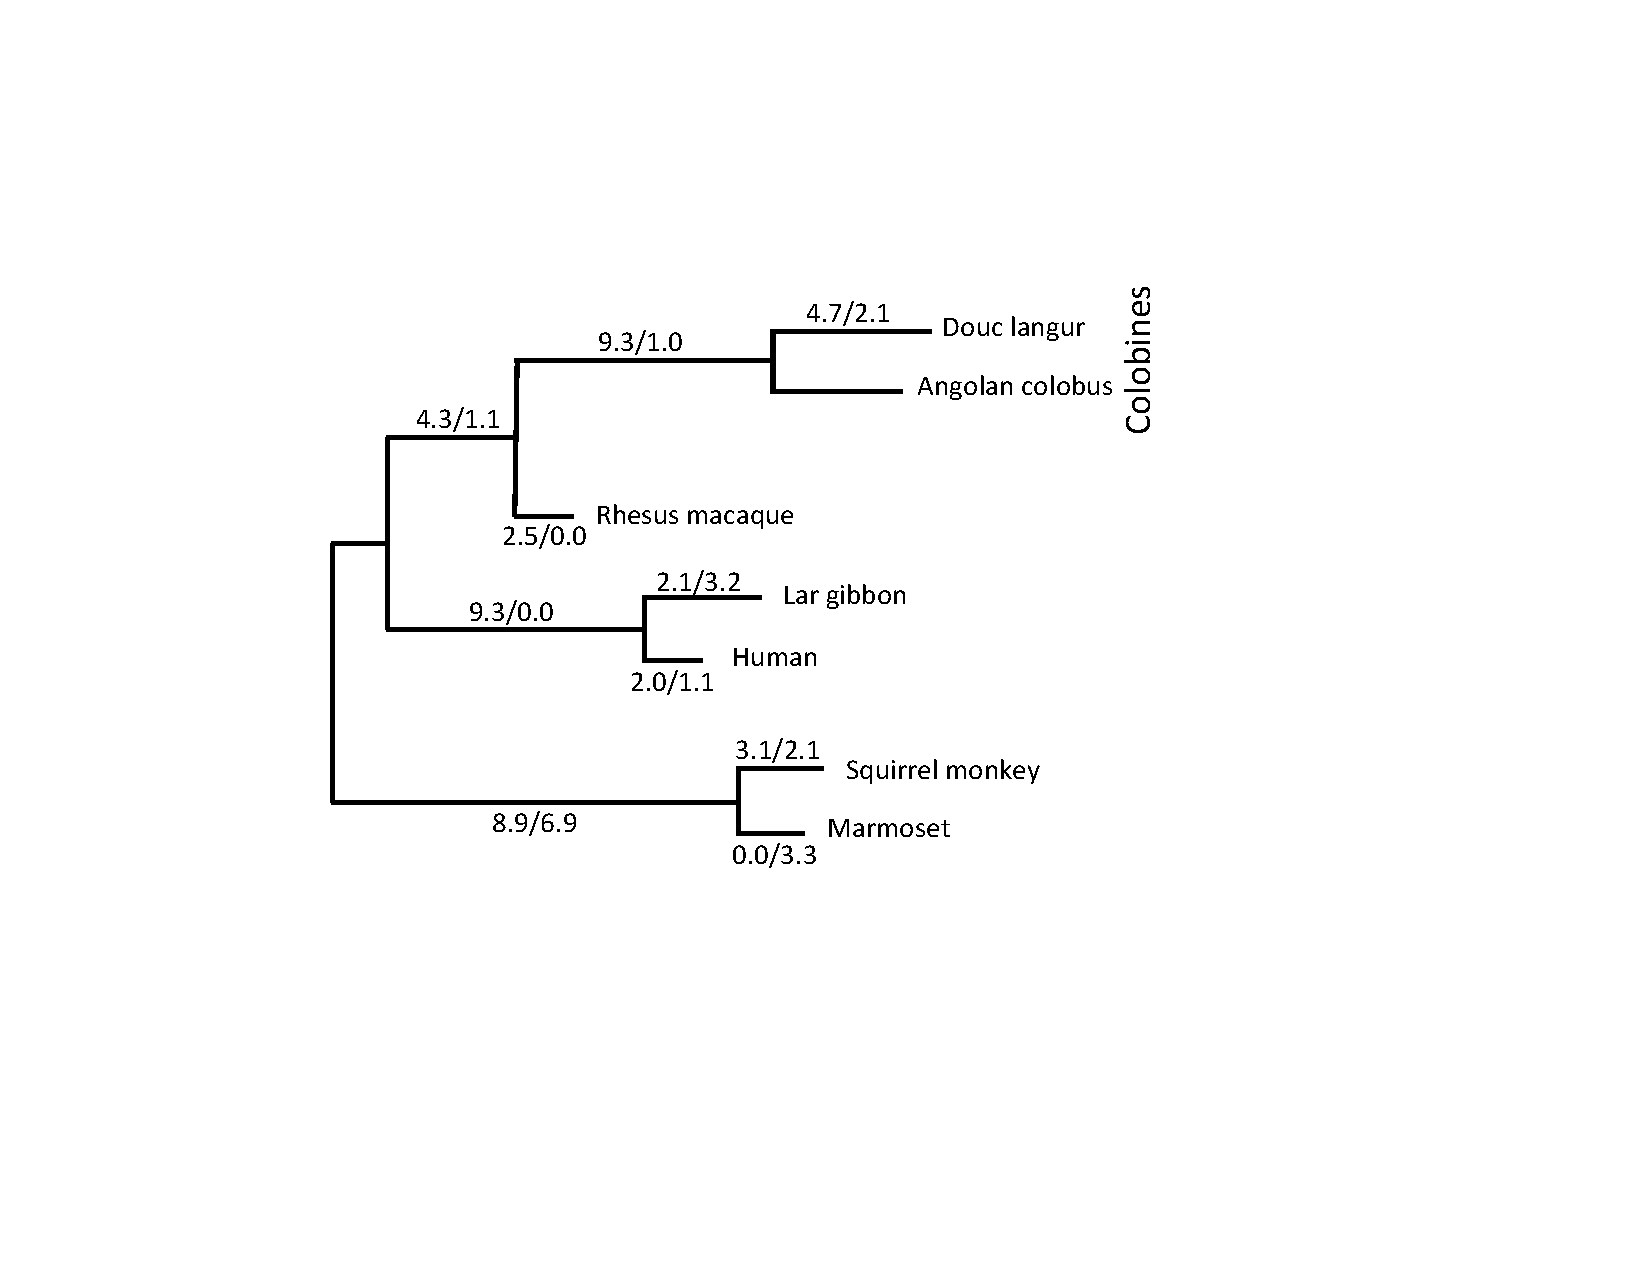
\includegraphics[width=0.8 \textwidth]{Journal_figs/genetic_drift/Yang_lysozyme/Yang_lysozyme.pdf}
\end{center}
\caption{A phylogram for the primate {\it lysozyme} gene, data from
  \citet{Yang:98}. For each branch, the numbers give the estimated average
number of non-synonymous to synonymous changes in the lysozyme protein.} \label{fig:lysozyme}
\end{figure}
%JRI: Angolan colobus missing numbers
\begin{marginfigure}
\begin{center}
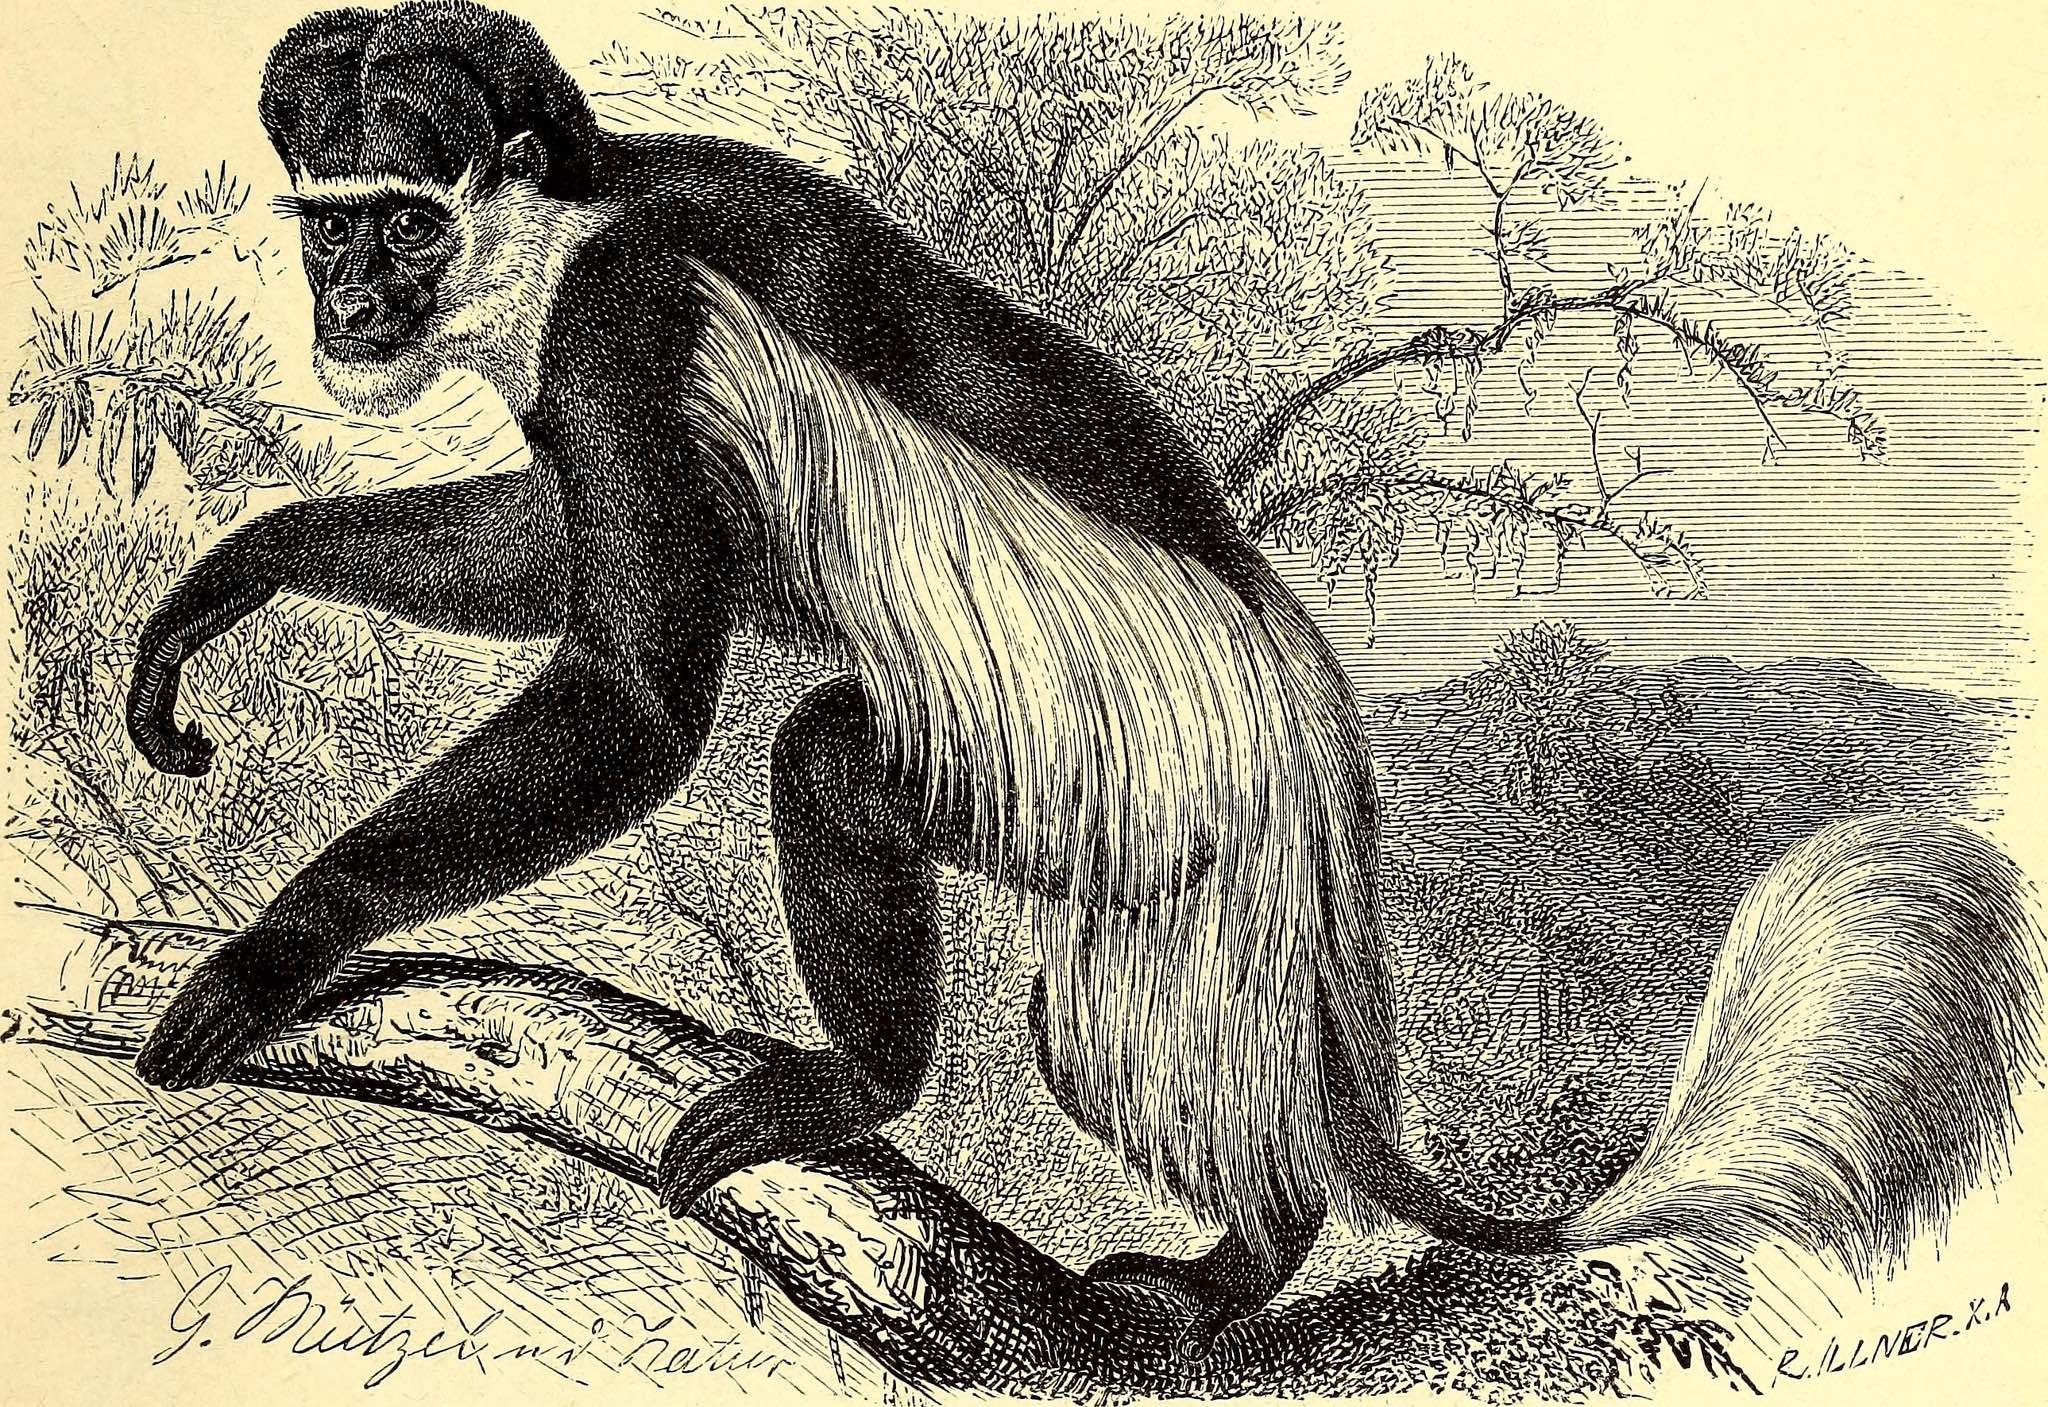
\includegraphics[width=0.8 \textwidth]{illustration_images/Genetic_drift/Colobus/19792029373_fcce706e67_k.jpg}
\end{center}
\caption{Abyssinian black-and-white colobus ({\it Colobus guereza}). A member of the leaf-eating Colobines. \BHLNC{Brehm's Tierleben,  Brehm,
  A.E. 1893.}{https://archive.org/stream/brehmstierlebena001breh/\#page/125/mode/1up}{University of Illinois Urbana-Champaign}} \label{fig:Colobus}
\end{marginfigure}


A classic example for looking at adaptive evolution using $\dNdS$ is the
evolution of the {\it lysozyme} gene in primates \citep{Messier:97,Yang:98}. The lysozyme protein is
a key component for the breakdown of bacterial walls. The {\it lysozyme} gene shows very
fast protein evolution (see
the phylogeny in Figure \ref{fig:lysozyme}), notably on the lineages leading to apes (e.g. gibbons
and humans) and Colobines (e.g. colobus and langur monkeys). Colobines have leaf-based diets. They digest
these leaves by bacterial fermentation in their foregut, and then use lysozymes to break down the bacteria to extract energy from the
leaves. In Colobines, the lysozyme protein has evolved to work well in the high-PH environment of the stomach. Remarkably, the Colobine
lysozyme protein has convergently evolved this activity via very similar amino-acid changes at 5 key residuals in cows and Hoatzins \citep[a leaf
eating bird,][]{kornegay1994molecular}
\begin{marginfigure}
\begin{center}
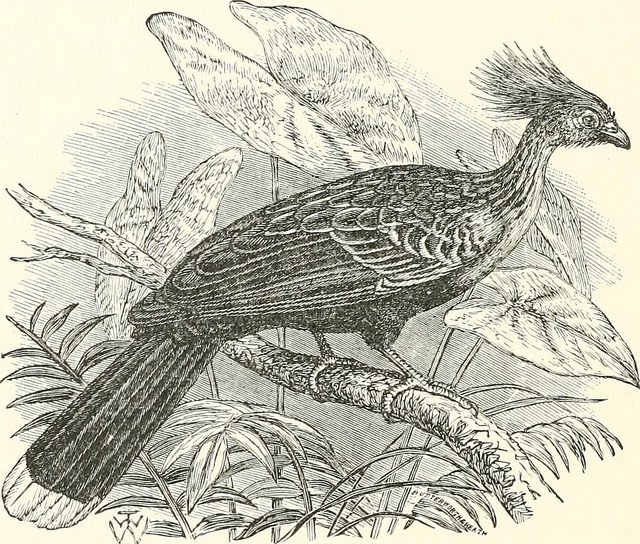
\includegraphics[width=0.8  \textwidth]{illustration_images/Genetic_drift/Hoatzin/14747388314_85798ba97e_z.jpg}
\end{center}
\caption{ (Hoatzin ({\it Opisthocomus hoazin}). A leaf-eating bird. \BHLNC{A history of birds (1910)
  Pycraft, W.P.}{https://archive.org/stream/historyofbirds00pycr/historyofbirds00pycr\#page/238/mode/1up}{ American Museum of Natural History Library}} \label{fig:hoatzin}
\end{marginfigure}
\paragraph{The McDonald-Kreitman test}

As noted above, a big issue with using $\dNdS$ to detect adaptation is that it is very conservative. For a more powerful test of rapid divergence, what we need to do is adjust for the level of constraint a gene experiences at non-synonymous sites. One way to do this is to use polymorphism data as an internal control. If we see little non-synonymous polymorphism at a gene, but a  lot of synonymous polymorphism, we now know that there is likely strong constraint on the gene (i.e. high $C$), thus we expect $\dNdS$ to be low. \citet{mcdonald:91} devised a simple test of the neutral theory of molecular evolution at a gene based on this intuition \citep[building on the conceptually similar HKA
test][]{hudson1987test}. \citeauthor{mcdonald:91} took the case where
we have polymorphism data at a gene for one species and divergence to
a closely related species. They  partitioned polymorphism and fixed
differences in their sample into the number of 
non-synonymous and synonymous changes:

\begin{center}
\begin{tabular}{ccc}
 & Poly. & Fixed \\
\hline
Non-Syn. &    $P_N$  &   $D_N$  \\
Syn. &    $P_S$   &     $D_S$   \\
Ratio & $P_N/P_S$ & $D_N/D_S$
\end{tabular}
\end{center}

\begin{marginfigure}
\begin{center}
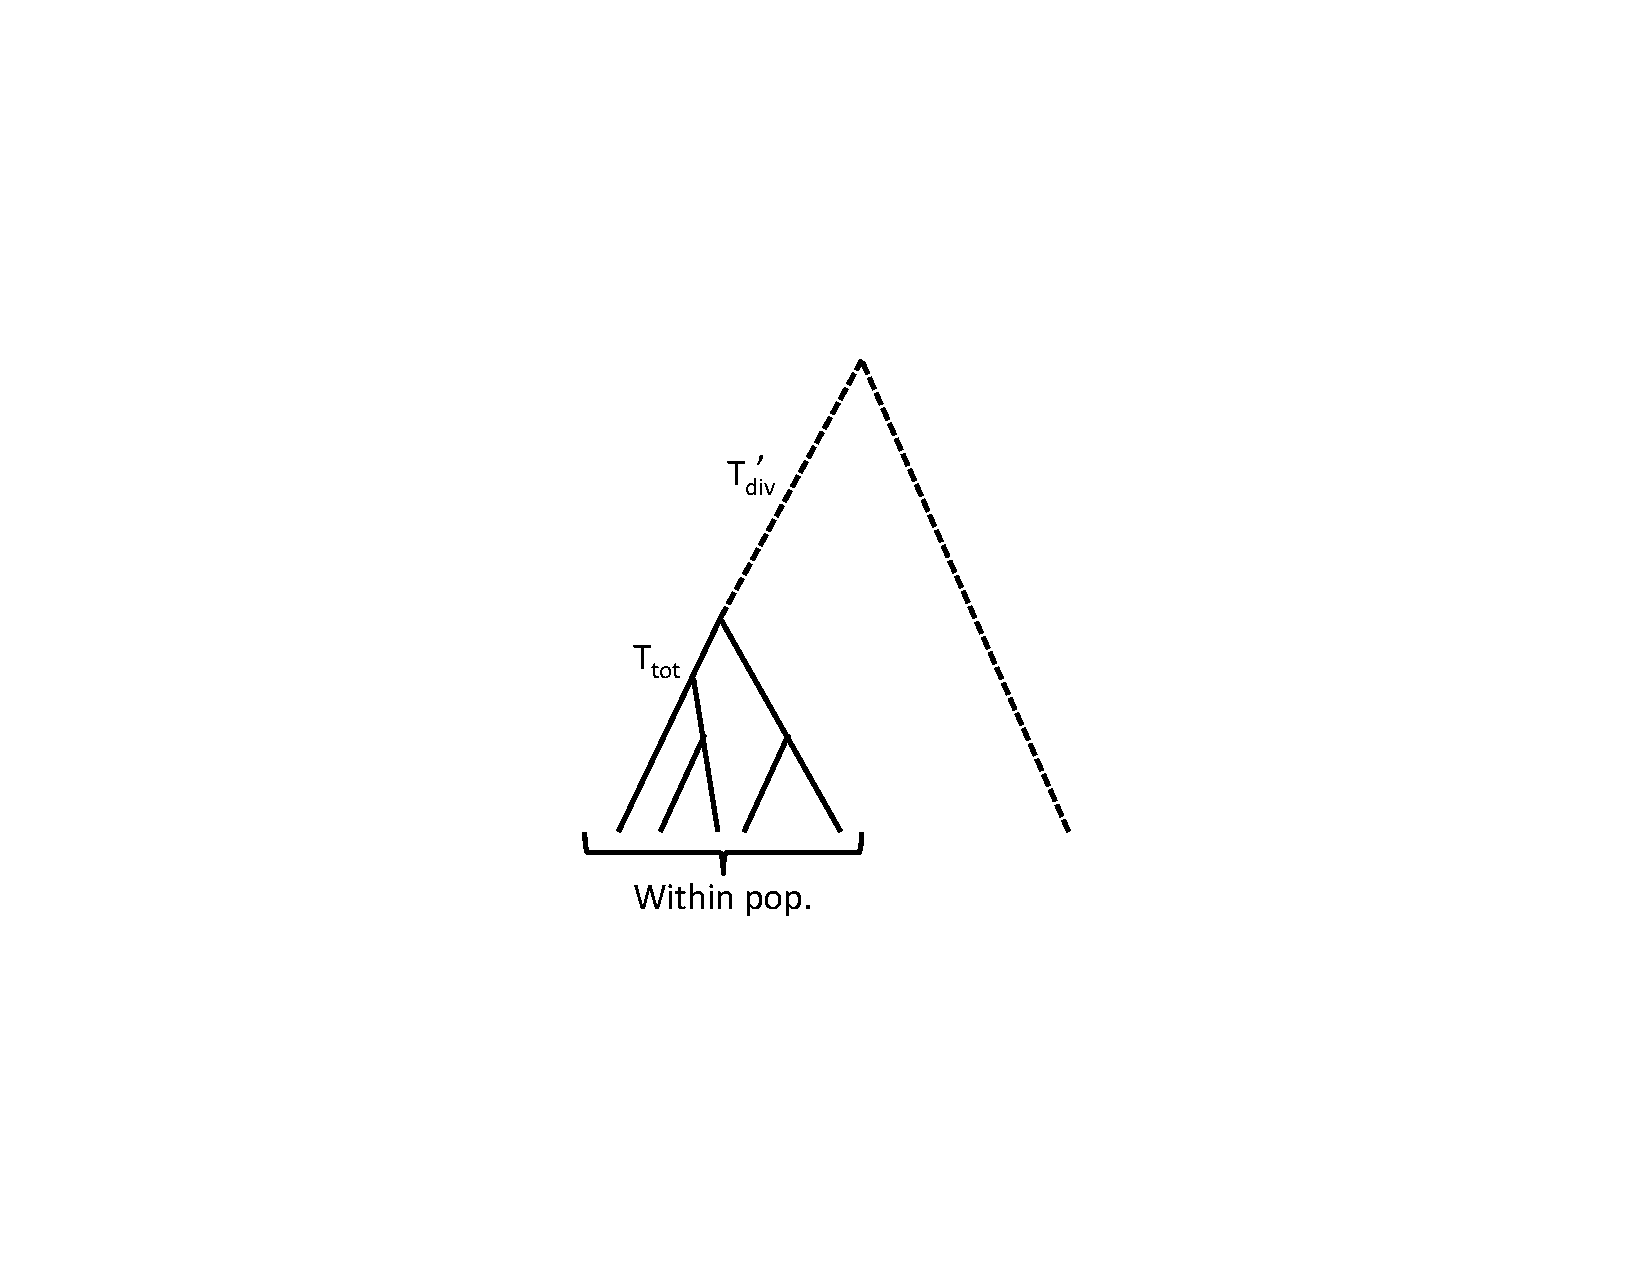
\includegraphics[width= \textwidth]{figures/Coalescent/MK_tree.pdf}
\end{center}
\caption{An example gene genealogy for a set of alleles sampled within
  a population and a single allele sampled from a distantly-related
  species. Here $T_{div}'$ is the total length of the dotted branch, we use 
  a $'$ on the T to indicate that this is not simply double the divergence
  time for the gene as the $T_{MRCA}$ for the sample has been
  subtracted off.} \label{fig:MK_tree}
\end{marginfigure}

Under neutral theory, we expect a smaller number of non-synonymous to
synonymous fixed differences ($D_N/D_S < 1$) and exactly the same
expectation holds for polymorphism ($P_N/P_S$). Let's consider a gene with $L_S$ and $L_N$ sites where synonymous and non-synonymous mutations could arise respectively.
We can think of the underlying gene genealogy at our gene, see Figure
\ref{fig:MK_tree}, with the total time on the coalescent genealogy
within the species as $T_{tot}$ and the total time for fixed
differences between our species as $T_{div}'$, note that $T_{div}'$ is
the total time where a an allele that would appear as a subsitution
could arise. Then under neutrality we expect $ \mu L_N (1-C) T_{tot}$
non-synonymous polymorphisms (i.e. our number of segregating sites), and  $ \mu L_N (1-C) T_{div}'$ non-synonymous fixed differences.
%JRI: maybe specify derived non-syn fixed diffs? as fixed differences between species an accrue on branch leading to outgroup as well, so more time than just T_{div}
We can then fill out the rest of our table as follows:

\begin{center}
\begin{tabular}{ccc}
 & Poly. & Fixed  \\
 \hline
Non-Syn. &    $\mu L_N (1-C) T_{tot}$  &   $\mu L_N (1-C)  T_{div}'$ \\
Syn. &    $\mu L_S T_{tot}$   &     $\mu L_S T_{div}'$  \\
Ratio & $ L_N(1-C)/( L_S)$  & $ L_N (1-C) / ( L_S)$
\end{tabular}
\end{center}
Therefore, we expect the ratio of non-synonymous to synonymous changes to be the same for polymorphism and divergence under a strict neutral model. We can test this expectation of equal ratios via the standard tests of a $2
\times 2$ table. If the ratio of $N/S$ is significantly higher for divergence than polymorphism we have evidence that non-synonymous substitutions are accumulating more rapidly than we would predict given levels of constraint alone.



% \begin{marginfigure}
% \begin{center}
% 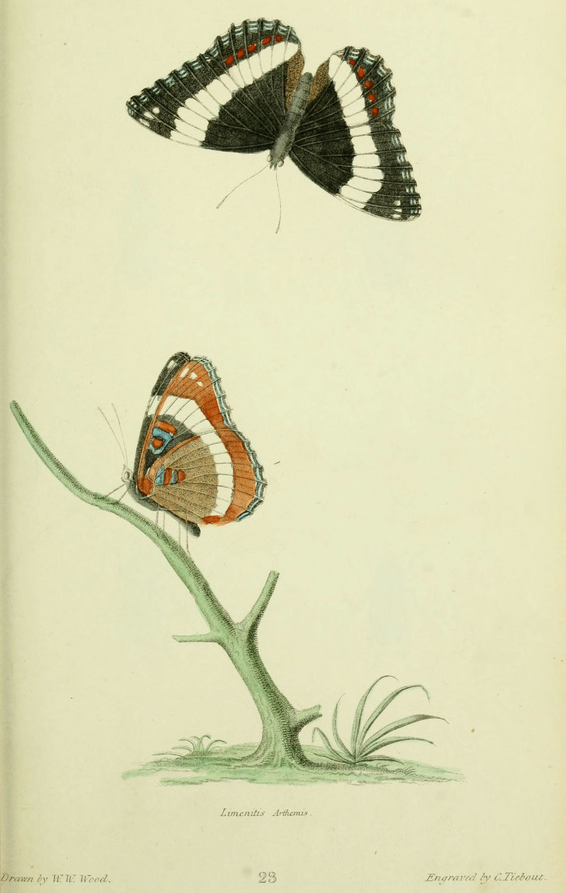
\includegraphics[width= \textwidth]{illustration_images/Genetic_drift/Limenitis_arthemis/Limenitis.png}
% \end{center}
% \caption{White admiral ({\it Limenitis arthemis}). \BHLNC{American entomology : a description of the insects of North American (1859). Say, T. }{https://www.biodiversitylibrary.org/page/9194935\#page/487/mode/1up}{Smithsonian Libraries}} \label{fig:Limenitis}
% \end{marginfigure}
As example of a Mcdonald-Kreitman (MK) table consider the work of \citet{frentiu2007adaptive} on the molecular evolution of L photopigment opsin in admiral
({\it Limenitis}) butterflies, responsible for colour vision in the
long-wavelength part of the visual
spectrum. \citeauthor{frentiu2007adaptive} found that the sensitivity
of this opsin had shifted towards blue in its sensitivity in {\it
  L. archippus archippus} (viceroy) compared to {\it  L. arthemis
  astyanax}. To test whether this molecular evolution reflected
positive selection they sequenced  24 {\it L. arthemis astyanax}
individuals and one {\it  L. archippus archippus} sequence. They
identified  11 polymorphic sites in  {\it L. arthemis astyanax} and 16
fixed differences, which break down as follows:
\begin{marginfigure}
\begin{center}
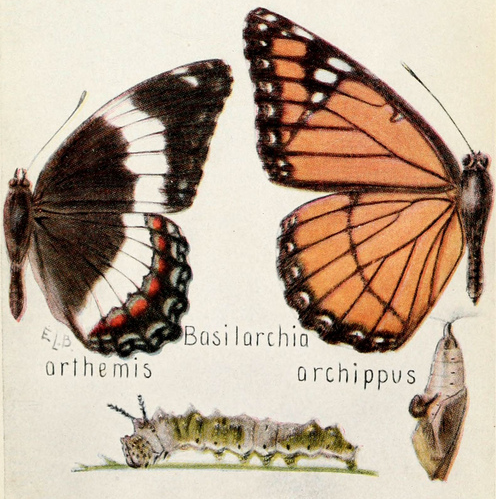
\includegraphics[width=\textwidth]{illustration_images/Genetic_drift/Basilarchia_arthemis_archippus/Basilarchia_arthemis_archippus.png}
\end{center}
\caption{White admiral ({\it Limenitis arthemis}) and viceroy ({\it
    Limenitis archippus}) butterflies.  {\it Basilarchia} is the old genus that these two species were originally placed in. Viceroy and monarch butterflies are M\"ullerian mimics. \BHLNC{Field book of insects (1918). Lutz, F.E. . illustrations by Edna L. Beutenm\"uller. }{https://www.flickr.com/photos/biodivlibrary/6244367298/in/photolist-avN2o3-avN1Eo-avN2gy-avN39b-avN1R9-avN2Hf-avN2CJ-avN2Um-avN1VS-avN3hU-avN2us-avN21m}{MBLWHOI Library}} \label{fig:Limenitis}
\end{marginfigure}
\begin{center}
\begin{tabular}{ccc}
 & Poly. & Fixed  \\
 \hline
Non-Syn. &    $2$  &   $12$ \\
Syn. &    $9$   &     $4$  \\
Ratio & $\nicefrac{2}{9}$  & $\nicefrac{3}{1}$
\end{tabular}
\end{center}
Note the strong excess of non-synonymous to synonymous divergence
compared to polymorphism (p-value of $0.006$, Fisher's exact test),
which is consistent with the gene evolving in an adaptive manner among
the two species. We would expect roughly only $3$ non-synonymous
substitutions out of 16 substitutions if the gene was evolving
neutrally ($ 16 \times \nicefrac{2}{11}$).

%We can then estimate the proportion of 


% \graham{add  Adriana Briscoe butterfly eye eg}  %https://twitter.com/AdrianaBriscoe/status/1057205734407094272


% We can push these ideas from the MK test further and try to estimate
% the proportion of subsitutions driven by positive selection.
% As in our simple model for the expected $\dNdS$, eqn \ref{eqn:dNDS_C_B},  we'll assume that there's only three
% classes of mutations, strongly deleterious, neutral, and
% beneficial. That gave us 

% Lets call this proportion $\alpha$, and our estimate of this quantity as 
% \begin{equation}
% \hat{\alpha} = 1 - \frac{D_S}{D_N}\frac{P_N}{P_S}
% \end{equation}
% To see why this is an estimate of the proportion of  Assume that there

\newpage
\begin{ChapterSummary}
\item In a diploid population of size $N$, any of a set of $2N$ selectively equivalent (ie neutral) alleles are equally likely to be the ancestor of the entire population at some future distant time point. Therefore, the probability that a new mutation eventually fixes in the population is $\nicefrac{1}{2N}$.
  \item Under a model where a fraction $C$ of new mutations are
    neutral and $1-C$ mutations are strongly deleterious, $2NC\mu$
    mutations arise every generation that can possibly become substitutions. Therefore, the per-generation rate of neutral substitution is $2N(1-C)\mu
    \times \nicefrac{1}{2N} = (1-C)\mu$. This is independent of the population size and just depends on levels of constraint and mutation rates.
  \item The constant rate of neutral substitution gives rise to a per-generation molecular clock, which can potentially be used to estimate constraint ($C$) and mutation rates.
    \item Many summaries and tests of molecular evolution, e.g. $\dNdS$, are based on comparing rates of substitution between functional classes of sites. These allow differing levels of constraint to be identified and signals of adaptive substitution to be detected. 
      \item Tests of molecular evolution for adaptation that also incorporate
        both divergence and polymorphism, e.g. the  Mcdonald-Kreitman
        test, are potentially powerful tools as polymorphism levels allow a somewhat independent measure of levels of constraint.  

      \end{ChapterSummary}


 \begin{question}{}
Assuming that the mutation rate is $\mu$/gamete/generation and the population size is N diploid individuals, what is the number of new mutations introduced into the population each generation?
\end{question}


\begin{question}{}
What is the probability of fixation of a unique new, neutral mutation in a population of N haploid individuals?
\end{question}

\begin{question}{}
Why is dN/dS much less than one for the majority of genes in our genome?
\end{question}

\begin{question}{}
You sequence a gene in {\it Drosophila melanogaster} and {\it D. simulans}. You
observe 5 non-synonymous substitutions out of 500 bases where
non-synonymous substitutions could occur, and 15 synonymous substitutions out of 500 bases where synonymous substitutions could
occur. What is the level of constraint at nonsynonymous sites?
\end{question}

\begin{question}{}
Analyzing polymorphism and divergence data for a gene, you calculate the
following McDonald-Kreitman table.
\begin{tabular}{lll}
 & Polymorp. & Fixed\\
Synonymous & 40 & 80  \\
Non-synonymous& 20 & 80\\
\end{tabular} \\
{\bf A)} Based on the ratio of non-synonymous to synonymous polymorphisms,
and given the 80 synonymous substitutions, how many nonsynymous
substitutions would you expect if this gene were evolving neutrally?\\
{\bf B)} Is this table consistent with the gene evolving neutrally? If not what could explain the results?
\end{question}
